%===============================================================================
% Authors: 2008 Michal Bidlo, 2018 Jaroslav Dytrych, 2019 Dominik Harmim
% Contact for questions and comments: dytrych@fit.vutbr.cz
% Author contact: xharmi00@stud.fit.vutbr.cz
%===============================================================================
% encoding: UTF-8
%------------------------------------------------------------------------------
% processing: make, make pdf, make clean
%==============================================================================
% Included files:
%  xharmi00-bibliography.bib - bibliography
%  xharmi00-chapters.tex - the thesis content
%  xharmi00-appendices.tex - appendices
%==============================================================================

\documentclass[english, czech, zadani, odsaz]{fitthesis}

% Basic packages are in template file fitthesis.cls.

% Setting of a path to the pictures.
\graphicspath{{figures/}{./figures/}}

\renewcommand{\ttdefault}{lmtt} % set Latin Modern tt as tt

% Disables function of the template which replaces quotation marks
% to avoid unnecessary replacements in the API descriptions etc.
\csdoublequotesoff

% "hyperref" package create clickable links in pdf if you are using pdflatex.
% Problem is that this package have to be introduced as the last one so it
% can not be placed in the template file.
\ifWis
    \ifx\pdfoutput\undefined % we are not using pdflatex
    \else
        \usepackage[
            unicode, colorlinks, hyperindex, plainpages=false, pdftex
        ]{hyperref}
        \definecolor{hrcolor-ref}{RGB}{223, 52, 30}
        \definecolor{hrcolor-cite}{HTML}{2F8F00}
        \definecolor{hrcolor-urls}{HTML}{092EAB}
        \hypersetup{
            linkcolor = hrcolor-ref,
            citecolor = hrcolor-cite,
            filecolor = magenta,
            urlcolor = hrcolor-urls
        }
        \def\pdfBorderAttrs{/Border [0 0 0]} % without margins around links
        \pdfcompresslevel=9
    \fi
\else % for the print clickable links will be black
    \ifx\pdfoutput\undefined % we are not using pdflatex
    \else
        \usepackage[
            unicode, colorlinks, hyperindex, plainpages=false, pdftex,
            urlcolor=black, linkcolor=black, citecolor=black
        ]{hyperref}
        \definecolor{links}{rgb}{0, 0, 0}
        \definecolor{anchors}{rgb}{0, 0, 0}
        \def\AnchorColor{anchors}
        \def\LinkColor{links}
        \def\pdfBorderAttrs{/Border [0 0 0]} % without margins around links
        \pdfcompresslevel=9
    \fi
\fi

% This solves the problems with links which leads after the picture.
\usepackage[all]{hypcap}

% solves first/last row of the paragraph on the previous/next page
\clubpenalty=10000
\widowpenalty=10000

\setlength{\parskip}{0pt}


% Information about the thesis
%-------------------------------------------------------------------------------
\projectinfo{
    % Thesis
    project = {BP}, % thesis type
    year = {2019}, % year of submission
    date = \today, % submission date
    faculty = {FIT}, % name of faculty
    department = {UITS}, % appropriate abbreviation of the department
%
    % Thesis title
    % thesis title in czech language
    title.cs = {%
        Statická analýza v~nástroji Facebook Infer zaměřená na detekci
        porušení atomičnosti
    },
    % thesis title in czech language for reference
    title.reference.cs = {%
        Statická analýza v~nástroji Facebook Infer zaměřená na detekci
        porušení atomičnosti.
    },
    % thesis title in english
    title.en = {%
        Static Analysis Using Facebook Infer to Find \\
        Atomicity Violations
    },
    % thesis title in english for reference
    title.reference.en = {%
        Static Analysis Using Facebook Infer to Find Atomicity Violations.
    },
%
    % Author
    author.name = {Dominik}, % author name
    author.surname = {Harmim}, % author surname
%
    % Supervisor
    supervisor.name = {Tomáš}, % supervisor name
    supervisor.surname = {Vojnar}, % supervisor surname
    supervisor.title.p = {prof. Ing.}, % title before the name
    supervisor.title.a = {Ph.D.}, % title after the name
%
    % Keywords
    % keywords in czech language
    keywords.cs = {%
        statická analýza, analýza programů, abstraktní interpretace,
        Facebook Infer, porušení atomicity, paralelní programy,
        kontrakty pro souběžnost, atomické sekvence, atomicita
    },
    % keywords in english
    keywords.en = {%
        static analysis, programs analysis, abstract interpretation,
        Facebook Infer, atomicity violation, concurrent programs,
        contracts for concurrency, atomic sequences, atomicity
    },
%
    % Abstract
    % abstract in czech language
    abstract.cs = {%
        Cílem této práce je navrhnout statický analyzátor programů pro detekci
        porušení atomicity. Navržený analyzátor\,---\,Atomer\,---\,je
        implementován jako rozšíření pro Facebook Infer, což je volně
        šířený a~snadno rozšířitelný nástroj, který umožňuje efektivní
        modulární a~inkrementální analýzu. Analyzátor pracuje na úrovni
        sekvencí volání funkcí. Navržené řešení je založeno na předpokladu,
        že sekvence, které jsou jednou zavolány atomicky, by měly být
        pravděpodobně volány atomicky vždy. Implementovaný analyzátor byl
        úspěšně ověřen a~vyhodnocen jak na malých programech, vytvořených
        pro tento účel, tak na veřejně dostupných testovacích programech,
        které vznikly ze skutečných nízko úrovňových programů.
    },
    % abstract in english
    abstract.en = {%
        The goal of this thesis is to propose a~static
        analyser of programs for detecting atomicity violations. The proposed
        analyser\,---\,Atomer\,---\,is implemented as an extension
        for Facebook Infer, which is an open-source and extendable static
        analysis framework that promotes efficient modular and incremental
        analysis. The analyser works on the level of sequences of function
        calls. The proposed solution is based on the assumption that
        sequences executed once atomically should probably be executed always
        atomically. The implemented analyser has been successfully verified
        and evaluated on both smaller programs created for this purpose as
        well as publicly available benchmarks derived from real-life low-level
        programs.
    },
%
    % Declaration
    declaration = {%
        Hereby I~declare that this bachelor’s thesis was prepared as an
        original author's work under the supervision of professor Tomáš Vojnar.
        All the relevant information sources, which were used during the
        preparation of this thesis, are properly cited and included in the
        list of references.
    },
%
    % Acknowledgement
    acknowledgment = {%
        I would like to thank my supervisor Tomáš Vojnar. Further, I would
        like to thank Tomáš Fiedor for providing supplementary information and
        for his assistance. I would also like to thank my colleagues Vladimír
        Marcin and Ondřej Pavela for helpful discussions about the thesis.
        Lastly, I thank for the support received from
        H2020 ECSEL project Aquas.
    }
}


\begin{document}
    % Typesetting of the title pages
    % --------------------------------------------------------------------------
    \maketitle


    % Table of contents
    % --------------------------------------------------------------------------
    {
        \hypersetup{hidelinks}
        \setcounter{tocdepth}{1}
        \tableofcontents
    }


    \ifODSAZ
        \setlength{\parskip}{0.5 \bigskipamount}
    \else
        \setlength{\parskip}{0pt}
    \fi


    % Skip the page in the two-sided mode
    \iftwoside\cleardoublepage\fi


    % Thesis text
    % --------------------------------------------------------------------------
    %===============================================================================
% (c) Dominik Harmim


%===============================================================================
\chapter{Introduction}

Bugs are an integral part of computer programs ever since the inception
of the programming discipline. Unfortunately, they are often hidden
in unexpected places, and they can lead to unexpected behaviour, which
may cause significant damage. Nowadays developers have many possibilities
of catching bugs in the early development process. \emph{Dynamic analysers}
or tools for automated testing are often used and they are satisfactory in 
many cases, nevertheless, they can still leave too many bugs undetected, 
because they are able to analyse only certain program flows dependent on 
the input data. An alternative solution is \emph{static analysis} that has 
its own shortcomings as well, such as the \emph{scalability} on extensive
codebases or considerably high rate of incorrectly reported errors 
(so-called \emph{false positives} or \emph{false alarms}).

Recently, Facebook introduced \emph{Facebook Infer}: a~tool for
creating \emph{highly scalable}, \emph{compositional}, \emph{incremental},
and \emph{interprocedural} static analysers. Facebook Infer has grown
considerably, but it is still under active development
by many teams across the globe. It is employed every day not only in
Facebook itself, but also in other companies, such as Spotify, Uber, Mozilla,
or Amazon. Currently, Facebook Infer provides several analysers that check 
for various types
of bugs, such as buffer overflows, data races and some forms of deadlocks
and starvation, null-dereferencing, or memory leaks. But most importantly
Facebook Infer is a~framework for building new analysers quickly and easily.
Unfortunately, the current version of Facebook Infer still lacks better 
support for \emph{concurrency} bugs. While it provides a~fairly advanced
\emph{data race} analyser, it is limited to Java and C++ programs only and 
fails for C~programs, which use a~more \emph{low-level} lock manipulation.

In \emph{concurrent programs}, there are often \emph{atomicity requirements}
for execution of specific sequences of instructions. Violating these
requirements may cause many kinds of problems, such as unexpected
behaviour, exceptions, segmentation faults, or other failures.
\emph{Atomicity violations} are usually not verified by compilers,
unlike syntactic or some sorts of semantic rules. Moreover, atomicity
requirements, in most cases, are not even documented at all. So in the
end, programmers themselves must abide by these requirements and usually
lack any tool support. And in general, it is difficult to avoid
errors in \emph{atomicity-dependent programs}, especially in large projects,
and even harder and time-consuming is finding and fixing them.

In this thesis, there is proposed the \emph{Atomer}\,---\,a~static
analyser for finding some forms of atomicity violations\,---\,which is
implemented as a~module of Facebook Infer. In particular, the stress 
is put on the \emph{atomic execution of sequences of function calls}, which is
often required, e.g., when using certain library calls. In fact, the idea
of checking atomicity of certain sequences of function calls is inspired
by the work of \emph{contracts for concurrency}~\cite{contracts2017}. In
the terminology of~\cite{contracts2017}, atomicity of certain sequences
of calls is the simplest (yet very useful in practice) kind of contracts 
for concurrency. The implementation particularly targets C/C++ programs 
that use \emph{PThread} locks.

The development of Atomer has been discussed with developers of
Facebook Infer, and it is a~part of the H2020 ECSEL project Aquas. Parts
of this thesis and preliminary results are taken from the
paper~\cite{excel2019FBInfer}, which was written in collaboration with 
Vladimír Marcin and Ondřej Pavela.

The rest of the thesis is organised as follows. In
Chapter~\ref{chap:prelim} there are described all the topics
which are necessary to understand before reading the rest of the thesis. In
particular, Section~\ref{sec:statAnalysisAI} deals with
\emph{static analysis} based on \emph{abstract interpretation}.
Facebook Infer, which uses abstract interpretation, is described in
Section~\ref{sec:fbinfer}. Finally, in Section~\ref{sec:contracts} there is
described the concept of \emph{contracts for concurrency}. A~proposal of
a~static analyser for detection of \emph{atomicity violations}, based on this
concept, is described in Chapter~\ref{chap:proposal} together with
a~description of existing analysers of a~similar kind. An implementation
of the analyser is presented in Chapter~\ref{chap:implement}. Subsequently,
Chapter~\ref{chap:exp} discusses the experimental evaluation of the analyser.
Finally, Chapter~\ref{chap:conc} concludes the thesis. In addition, there are
three appendices. Appendix~\ref{app:expRes} provides more details of 
experimental verification results. Appendix~\ref{app:memMedia} lists contents 
of the attached memory media, and Appendix~\ref{app:man} serves as an 
installation and user manual.



%===============================================================================
\chapter{Preliminaries}
\label{chap:prelim}

This chapter explains the theoretical background that the thesis builds
on. It also explains and describes the existing tools used in the
thesis. Lastly, the chapter deals with principles which this thesis
got inspired by.

In particular, in Section~\ref{sec:statAnalysisAI}, there is a~brief 
explanation of \emph{static analysis} itself, and then an explanation of
\emph{abstract interpretation} that is used in Facebook Infer, i.e., the
tool that is extended in this thesis. Facebook Infer, its principles and
features are illustrated in Section~\ref{sec:fbinfer}. The concept of
\emph{contracts for concurrency} that the thesis gets inspired by is
discussed and defined in Section~\ref{sec:contracts}.


\section{Static Analysis by Abstract Interpretation}
\label{sec:statAnalysisAI}

According to~\cite{staticAnalysisMoller}, \emph{static analysis} of
programs is reasoning about the behaviour of computer programs without
actually executing them. It has been used since the 1970s in optimising
compilers for generating efficient code. More recently, it has proven
valuable also for automatic error detection, verification of correctness 
of programs, and it is used in other tools that can help programmers.
Intuitively, a~static program analyser is a~program that reasons about the
behaviour of other programs, in other words, a~static program analyser is
a~program that reasons about another programs by looking for some
\emph{syntactic patterns} in the code and/or by assigning the program
statements some \emph{abstract semantics} and then deriving
a~characterisation of the behaviour in terms of the abstract semantics.
Nowadays, static analysis is one of the fundamental concepts of 
\emph{formal verification}. It aims to automatically answer questions 
about a~given program, such as, e.g.,~\cite{staticAnalysisMoller}:
\begin{itemize}
    \item
        \textbf{Are certain operations executed \emph{atomically}?}

    \item
        Does the program terminate on every input?

    \item
        Can the program \emph{deadlock}?

    \item
        Does there exist an input that leads to a~\emph{null-pointer
        dereference}, a~\emph{division-by-zero}, or an \emph{arithmetic
        overflow}?

    \item
        Are all variables initialised before they are used?

    \item
        Are arrays always accessed within their bound?

    \item
        Does the program contain \emph{dead code}?

    \item
        Are all resources correctly released after their last
        use?
\end{itemize}

It is well-known that testing, i.e., executing programs
with some input data and examining the output, may expose errors, but it
cannot prove their absence. (It was also famously stated by Edsger W.
Dijkstra: \uv{\textit{Program testing can be used to show the presence of bugs,
but never to show their absence!}}.) However, static program analysis
can prove their absence\,---\,with some \emph{approximation}\,---\,it can
check \emph{all possible executions} of the programs and provide guarantees
about their properties. Another advantage of static analysis is that the
analysis can be performed during the development process, so the program
does not have to be executable yet and it already can be analysed.
The biggest disadvantage of static analysis is that it can produce many
\emph{false alarms}\footnote{\textbf{False alarms}\,--\,incorrectly reported 
an error. Also called \emph{false positives}.}, which is often resolved by
accepting \emph{unsoundness}\footnote{\textbf{Soundness}\,--\,if 
a~verification method claims that a~system is correct according to a~given
specification, it is truly correct~\cite{favStaticAnalysis}.}. Another major
issue is that of ensuring sufficient \emph{scalability} of static analysis: 
in fact, typically, the more precise the analysis is, the less scalable it
becomes.

Various forms of static analysis of programs have been invented, for
instance~\cite{favStaticAnalysis}: bug pattern searching, data-flow
analysis, constraint-based analysis, type analysis, or symbolic execution.
One of the most widely used approaches\,---\,\emph{abstract
interpretation}\,---\,is detailed in Section~\ref{sec:AI}.

There exist numerous tools for static analysis (often proprietary and
difficult to openly evaluate or extend), e.g.: Coverity, Klockwork, CodeSonar,
Frama-C, PHPStan, or \emph{Facebook Infer} (described in
Section~\ref{sec:fbinfer}).


\subsection{Abstract Interpretation}
\label{sec:AI}

This section explains and defines the basics of \emph{abstract interpretation}.
The description is based on~\cite{AIBasedFormalMethodsCousot,
AILatticeModelCousot, AIInNutshellCousot, AICousotWeb, favAI,
projectPracticeMarcin2018, wideningNarrowingCousot, programAnalysisNielson,
staticAnalysisMoller, favLatticesAndFixpoints}. In these works, there can be
found more detailed and more formal explanation.

Abstract interpretation was introduced and formalised by a~French
computer scientist Patrick Cousot and his wife Radhia Cousot in the year
1977 at POPL (symposium on Principles of Programming
Languages)~\cite{AILatticeModelCousot}. It is a~generic \emph{framework}
for static analyses. It allows one to create particular analyses by
providing specific components (described later) to the framework. The
obtained analysis is guaranteed to be \emph{sound} if certain properties 
of the components are met.~\cite{favAI, projectPracticeMarcin2018}

In general, in the set theory, which is independent of the application
setting, abstract interpretation is considered a~theory for
\emph{approximating} sets and set operations. A~more restricted formulation
of abstract interpretation is to interpret it as a~theory of approximation
of the behaviour of the \emph{formal semantics} of programs. Those
behaviours may be characterised by \emph{fixpoints} (defined below), which 
is why a~primary part of the theory provides efficient techniques for
\emph{fixpoint approximation}~\cite{programAnalysisNielson}.
So, for a~standard semantics, abstract interpretation is used to derive
the approximate abstract semantics over an \emph{abstract domain} (defined
below). The abstract semantics obtained as a~result of program analysis can 
then be used for verification, optimisation, code generation or 
transformation, etc.~\cite{AIBasedFormalMethodsCousot}

Patrick Cousot intuitively and informally illustrates abstract
interpretation in~\cite{AIInNutshellCousot} as follows.
Figure~\ref{fig:ai1} shows the \emph{concrete semantics} of a~program
by a~set of curves, which represents the set of all possible executions
of the program in all possible execution environments. Each curve shows
the evolution of the vector~$ x(t) $~of input values, state, and
output values of the program as a~function of the time~$ t $.
\emph{Forbidden zones} on this figure represent a~set of erroneous states
of the program execution. Proving that the intersection of the concrete
semantics of the program with the forbidden zone is empty may be
\emph{undecidable} because the program concrete semantics is, in general, 
\emph{not computable}. As demonstrates Figure~\ref{fig:ai2}, abstract
interpretation deals with an \emph{abstract semantics}, i.e., the
\emph{superset} of the concrete program semantics. The abstract semantics
includes all possible executions. That implies that if the abstract 
semantics is safe (i.e. it does not intersect the forbidden zone), the 
concrete semantics is safe as well. However, the \emph{over-approximation} 
of the possible program executions causes that inexisting program executions 
are considered, which may lead to \emph{false alarms}. It is the case when 
the abstract semantics intersects the forbidden zone, whereas the concrete 
semantics does not intersect it.

\begin{figure}[hbt]
    \centering

    \begin{subfigure}[hbt]{.45 \linewidth}
        \centering
        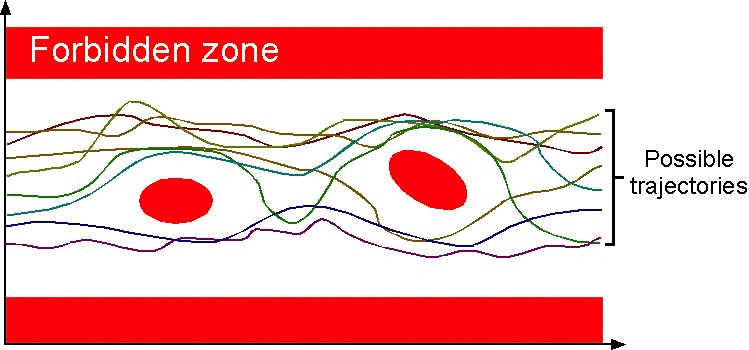
\includegraphics[width=1 \linewidth]{ai_1.png}
        \caption{%
            \emph{Concrete semantics} of programs with
            \emph{forbidden zones}
        }
        \label{fig:ai1}
    \end{subfigure}
%
    \hfill
%
    \begin{subfigure}[hbt]{.45\linewidth}
        \centering
        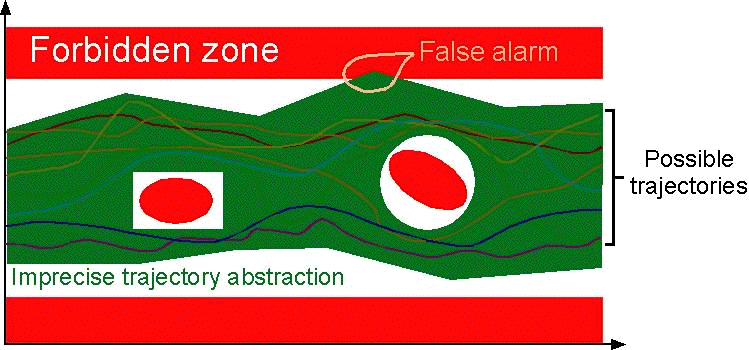
\includegraphics[width=1 \linewidth]{ai_2.png}
        \caption{%
            \emph{Abstract semantics} of programs with imprecise
            trajectory abstraction
        }
        \label{fig:ai2}
    \end{subfigure}

    \caption{%
        Abstract interpretation demonstration~\cite{AIInNutshellCousot}.
        Horizontal axes: time~$ t $. Vertical axes:
        vector~$ x(t) $~of input, state, and output values of the
        considered program
    }
\end{figure}

\subsubsection{Components of Abstract Interpretation}

In accordance with~\cite{favAI, projectPracticeMarcin2018}, the basic 
components of abstract interpretation are as follows:
\begin{itemize}
    \item
        \textbf{An Abstract Domain}~\cite{AICousotWeb}:

        \begin{itemize}
            \item
                An abstraction of the possible concrete program states
                (or their parts) in the form of \emph{abstract
                properties}\footnote{\textbf{Abstract properties} 
                approximating \emph{concrete properties behaviours}.} 
                and \emph{abstract operations}\footnote{\textbf{Abstract
                operations} include abstractions of the \emph{concrete
                approximation}, an approximation of the \emph{concrete 
                fixpoint transform function},
                etc.}~\cite{AIBasedFormalMethodsCousot}.

            \item
                Sets of program states at certain locations are represented
                using \emph{abstract states}.
        \end{itemize}

    \item 
        \textbf{Abstract Transformers}:

        \begin{itemize}
            \item
                There is a~\emph{transform function} for each program
                operation (instruction) that represents the impact
                of the operation executed on an abstract state.
        \end{itemize}

    \item 
        \textbf{The Join Operator}~$ \circ $:

        \begin{itemize}
            \item
                Joins abstract states from individual program branches into
                a~single one.
        \end{itemize}

    \item
        \textbf{The Widening
        Operator~$ \triangledown $}~\cite{programAnalysisNielson,
        wideningNarrowingCousot, favAI}:

        \begin{itemize}
            \item
                Enforces termination of the abstract interpretation.

            \item
                It is used to approximate the \emph{least fixed points}
                of program semantics (it is performed on a~sequence of 
                abstract states at a~certain location).

            \item
                Usually, the later in the analysis this operator is used, 
                the more accurate the result is (but the analysis takes more
                time).
        \end{itemize}

    \item
        \textbf{The Narrowing
        Operator~$ \vartriangle $}~\cite{programAnalysisNielson,
        wideningNarrowingCousot, favAI}:

        \begin{itemize}
            \item
                Using this operator, the approximation obtained by
                widening can be refined, i.e., it may be used to refine the
                result of widening.

            \item
                This operator is used when a~\emph{fixpoint} is
                approximated using widening.
        \end{itemize}
\end{itemize}

\subsubsection{Fixpoints and Fixpoint Approximation}

A~\textbf{fixpoint} of a~function  $ f : A \rightarrow A $ is an
element $ a \in A $ if and only if 
$ \boldsymbol{f(a) = a} $~\cite{favLatticesAndFixpoints}.

Computation of the \emph{most precise abstract fixpoint} is not generally
guaranteed to terminate, in particular, when a~given program contains
a~loop or recursion. The solution is to approximate the fixpoint using
\emph{widening} (over-approximation of a~fixpoint) and \emph{narrowing}
(improves the approximation of the fixpoint)~\cite{favAI,
projectPracticeMarcin2018}. Most program properties can be represented as
fixpoints. This reduces program analysis to the fixpoint
approximation~\cite{AICousotWeb}. Further information about fixpoint
approximation can be found, e.g., in~\cite{programAnalysisNielson,
wideningNarrowingCousot}.

\subsubsection{Formal Definition of Abstract Interpretation}

According to~\cite{AILatticeModelCousot, favAI},
\textbf{abstract interpretation}~$ \boldsymbol{I} $~of a~program~$ P $~with
the instruction set~$ S $~is a~tuple
$$ \boldsymbol{I = (Q, \circ, \sqsubseteq, \top, \bot, \tau)} $$
where
\begin{itemize}
    \item
        $ \boldsymbol{Q} $~is the \emph{abstract domain} (domain of
        \emph{abstract states}),

    \item
        $ \boldsymbol{\circ}~\text{:}~Q \times Q \rightarrow Q $
        is the \emph{join operator} for accumulation of abstract states,

    \item
        $ \text{(}\boldsymbol{\sqsubseteq}\text{)} \subseteq Q \times Q $ is
        an \emph{ordering} defined as
        $ x \sqsubseteq y \Leftrightarrow x \circ y = y $ in
        $ (Q, \circ, \top) $,

    \item
        $ \boldsymbol{\top} \in Q $ is the \emph{supremum} of~$ Q $,

    \item
        $ \boldsymbol{\bot} \in Q $ is the \emph{infimum} of~$ Q $,

    \item
        $ \boldsymbol{\tau}~\text{:}~S \times Q \rightarrow Q $
        defines \emph{abstract transformers} for specific instructions,

    \item
        $ (Q, \circ, \top) $ is a~\emph{complete
        semilattice}~\cite{favLatticesAndFixpoints, favAI}.
\end{itemize}

Using so-called \emph{Galois connections}~\cite{programAnalysisNielson,
wideningNarrowingCousot, favAI, AICousotWeb}, one can guarantee the
\emph{soundness} of abstract interpretation.


\section{\texorpdfstring{Facebook Infer\,---\,A~Static Analysis Framework}{}}
\label{sec:fbinfer}

This section describes the principles and features of
\emph{Facebook Infer}. The description is based on information provided
at the Facebook Infer website\footnote{\textbf{Facebook Infer}
website\,--\,\url{https://fbinfer.com}.} and in~\cite{inferAISlides,
projectPracticeMarcin2018}. Parts of this section are taken
from the paper~\cite{excel2019FBInfer}.

Facebook Infer is an open-source\footnote{\textbf{Open-source repository of
Facebook Infer} on GitHub\,--\,\url{https://github.com/facebook/infer}.}
static analysis \emph{framework}, which is able to discover various kinds of
software bugs of a~given program, with the stress put on \emph{scalability}.
The basic usage of Facebook Infer is illustrated in Figure~\ref{fig:infer}.
A~more detailed explanation of its architecture is shown below. Facebook 
Infer is implemented in \emph{OCaml}\footnote{\textbf{OCaml}
website\,--\,\url{https://ocaml.org}.}\,--\,\emph{functional} programming
language, also supporting \emph{imperative} and \emph{object-oriented}
paradigms. Further details about OCaml can be found in~\cite{realWorldOCaml}
or in official documentation\footnote{\textbf{OCaml
documentation}\,--\,\url{http://caml.inria.fr/pub/docs/manual-ocaml}.},
tutorials\footnote{\textbf{OCaml
tutorials}\,--\,\url{https://ocaml.org/learn/tutorials}.}. Facebook Infer was
originally a~standalone tool focused on \emph{sound verification} of the 
absence of \emph{memory safety violations}, which was first published in
the well-known paper~\cite{inferBiabduction}.

\begin{figure}[hbt]
    \centering
    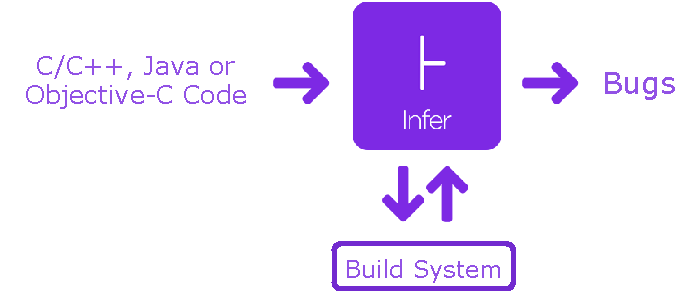
\includegraphics[width=.7 \linewidth]{infer.pdf}
    \caption{%
        Static analysis in Facebook Infer
        (\url{%
            http://www.codeandyou.com/2015/06/%
            infer-static-analyzer-for-java-c-and.html%
        })
    }
    \label{fig:infer}
\end{figure}

Facebook Infer is able to analyse programs written in several languages.
In particular, it supports languages C, C++, Java, and Objective-C. Moreover,
it is possible to extend Facebook Infer's \emph{frontend} for supporting
other languages. Currently, Facebook Infer contains many analyses focusing
on various kinds of bugs, e.g., \emph{Inferbo} (buffer
overruns)~\cite{inferboOnline}; \emph{RacerD} (data races)~\cite{racerD,
racerDOnline, staticRaceDetectorTruePositive}; and other analyses
that check for buffer overflows, some forms of deadlocks and starvation,
null-dereferencing, memory leaks, resource leaks, etc.


\subsection{Abstract Interpretation in Facebook Infer}
\label{sec:fbinferAI}

Facebook Infer is a~general framework for static analysis of programs, it is
based on \emph{abstract interpretation}. Despite the original approach 
taken from~\cite{inferBiabduction}, Facebook Infer  aims to find bugs rather
than formal verification. It can be used to quickly develop new sorts of
\emph{compositional} and \emph{incremental} analysers (\emph{intraprocedural} 
or \emph{interprocedural}~\cite{programAnalysisNielson}) based
on the concept of function \emph{summaries}. In general, a~\emph{summary}
is a~representation of \emph{preconditions} and \emph{postconditions} of
a~function. However, in practice, a~summary is a~custom data structure that
may be used for storing any information resulting from the analysis of
particular functions. Facebook Infer generally does not compute the summaries
in the course of the analysis along the \emph{Control Flow Graph}
(\textbf{CFG})\footnote{\textbf{A~control flow graph (CFG)} is a~directed
graph in which the nodes represent basic blocks and the edges represent control
flow paths~\cite{controlFlowAnalysisAllen}.} as it is done in classical
analyses based on the concepts from~\cite{dataflowAnalysisGraphReachability,
dataflowAnalysisApproaches}. Instead, Facebook Infer performs the
analysis of a~program \emph{function-by-function along the call tree},
starting from its leafs (demonstrated later). Therefore, a~function
is analysed and a~summary is computed without knowledge of the
call context. Then, the summary of a~function is used at all of its call 
sites. Since summaries do not differ for different contexts, the analysis
becomes more scalable, but it can lead to a~loss of accuracy. In order 
to create a~new intraprocedural analyser in Facebook Infer, it is needed to 
define the following (listed items are described in more detail in
Section~\ref{sec:AI}):
\begin{enumerate}
    \item
        The \emph{abstract domain}~$ Q $, i.e., a~type of an
        \emph{abstract state}.

    \item
        Operator~$ \sqsubseteq $, i.e., an \emph{ordering} of abstract
        states.

    \item
        The \emph{join} operator~$ \circ $, i.e., the way of joining two
        abstract states.

    \item
        The \emph{widening} operator~$ \triangledown $, i.e., the way how to
        enforce termination of the abstract interpretation of an iteration.

    \item
        \emph{Transfer functions}~$ \tau $, i.e., a~transformer that
        takes an abstract state as an input and produces an abstract state
        as an output.
\end{enumerate}
Further, in order to create an interprocedural analyser, it is required to
additionally define:
\begin{enumerate}
    \item
        The type of function summaries.

    \item
        The logic for using summaries in transfer functions, and the logic
        for transforming an intraprocedural abstract state to
        a~summary.
\end{enumerate}
An important feature of Facebook Infer improving its scalability is
\emph{incrementality} of the analysis, it allows one to analyse separate
code changes only, instead of analysing the whole codebase. It is more
suitable for extensive and variable projects, where ordinary analysis
is not feasible. The incrementality is based on \emph{re-using summaries}
of functions for which there is no change in them neither in the functions
transitively invoked from them.

\subsubsection{%
    The Architecture of the Abstract Interpretation Framework in
    Facebook Infer
}

The architecture of the abstract interpretation framework of Facebook
Infer (\textbf{Infer.AI}) may be split into three major parts,
as demonstrated in Figure~\ref{fig:inferArch}: a~\emph{frontend},
an \emph{analysis scheduler} (and a~\emph{results database}), and a~set of
\emph{analyser plugins}.

The frontend compiles input programs into the \emph{Smallfoot Intermediate
Language} (SIL) and represents them as a~CFG. There is a~separate CFG
representation for each analysed function. Nodes of this CFG are formed as
instructions of SIL. The SIL language consists of the following underlying
instructions:
\clearpage
\begin{itemize}
    \item
        \texttt{LOAD}: reading into a~temporary variable.

    \item
        \texttt{STORE}: writing to a~program variable,
        a~field of a~structure, or an array.

    \item
        \texttt{PRUNE~e}~(often called \texttt{ASSUME}): 
        evaluation of a~condition~\texttt{e}.

    \item
        \texttt{CALL}: a~function call.
\end{itemize}
The frontend allows one to propose \emph{language-independent} analyses
(to a~certain extent) because it supports input programs to be written
in multiple languages.

\begin{figure}[hbt]
    \centering
    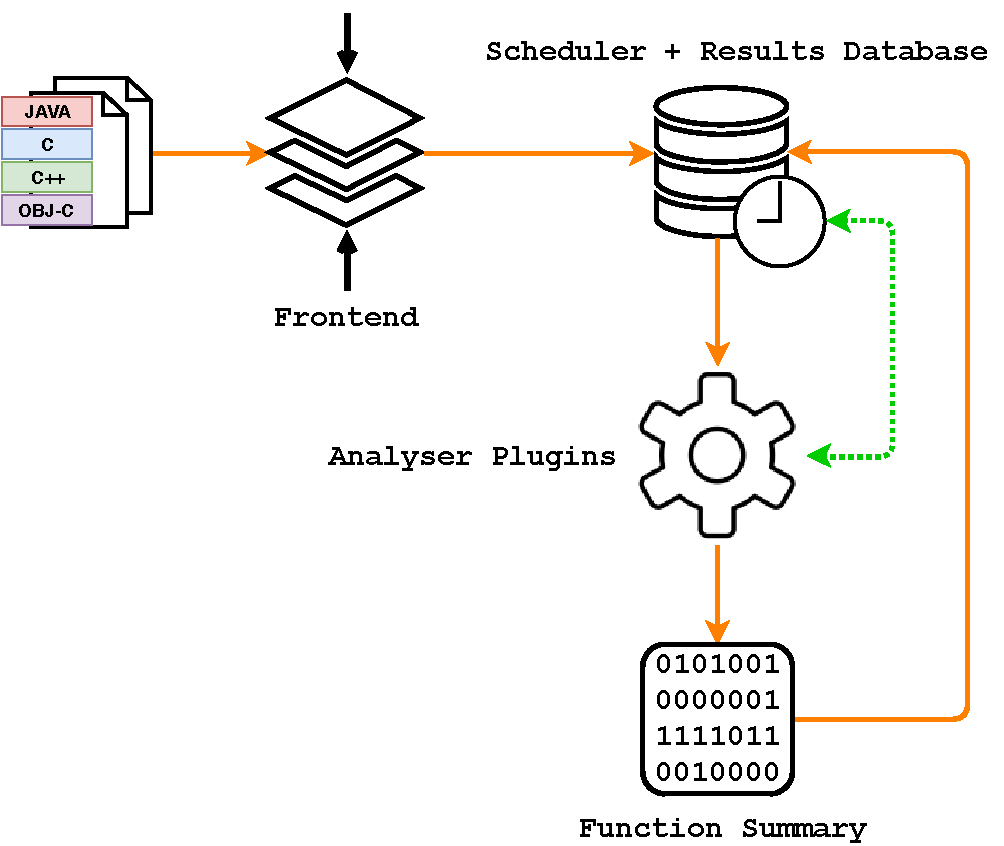
\includegraphics[width=.65 \linewidth]{infer_architecture.pdf}
    \caption{%
        The architecture of Facebook Infer's abstract interpretation
        framework~\cite{inferAISlides, projectPracticeMarcin2018}
    }
    \label{fig:inferArch}
\end{figure}

\begin{wrapfigure}{r}{.45 \linewidth}
    \centering
    \vspace{-1em}
    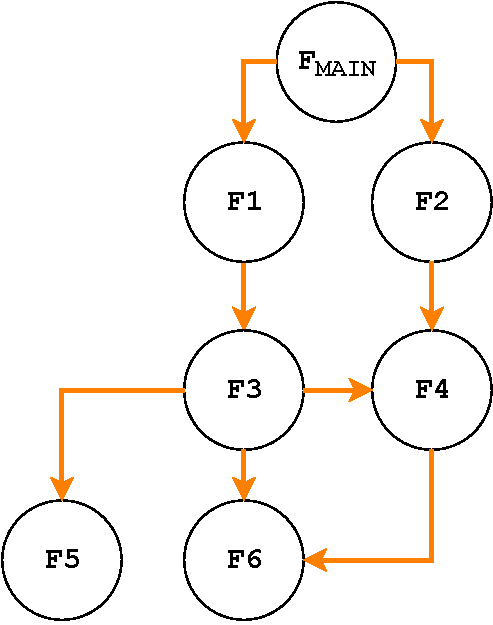
\includegraphics[width=.25 \textwidth]{infer_call_graph.pdf}
    \caption{%
        A~call graph for an illustration of Facebook Infer's
        analysis process~\cite{inferAISlides, excel2019FBInfer,
        projectPracticeMarcin2018}
    }
    \label{fig:inferCallGraph}
\end{wrapfigure}
The next part of the architecture is the scheduler, which defines the
order of the analysis of single functions according to the appropriate
\emph{call graph}\footnote{\textbf{A~call graph} is a~\emph{directed graph}
describing call dependencies among functions.}. The scheduler also checks
if it is possible to analyse some functions simultaneously, which allows
Facebook Infer to run the analysis in parallel.

\begin{example}
    For demonstrating the order of the analysis in Facebook Infer and its
    incrementality, assume a~call graph in Figure~\ref{fig:inferCallGraph}.
    At first, leaf functions \texttt{F5} and \texttt{F6} are analysed. 
    Further, the analysis goes on towards the root of the call
    graph\,--\,\texttt{F\textsubscript{MAIN}}, while taking into 
    consideration the dependencies denoted by the edges. This order ensures 
    that a~summary is available once a~nested function call is abstractly
    interpreted within the analysis. When there is a~subsequent code change,
    only directly changed functions and all the functions up the call path 
    are re-analysed. For instance, if there is a~change of source code of
    function \texttt{F4}, Facebook Infer triggers re-analysis of 
    functions \texttt{F4}, \texttt{F2}, and \texttt{F\textsubscript{MAIN}} 
    only.
\end{example}

The last part of the architecture consists of a~set of analyser plugins.
Each plugin performs some analysis by interpreting of SIL instructions.
The result of the analysis of each function (function summary) is stored to
the results database. The interpretation of SIL instructions (\emph{commands})
is done using an \emph{abstract interpreter} (also called a~\emph{control
interpreter}) and \emph{transfer functions} (also called a~\emph{command
interpreter}). The transfer functions take an actual \emph{abstract state}
of an analysed function as an input, and by applying the interpreting command,
produce a~new abstract state. The abstract interpreter interprets the
command in an \emph{abstract domain} according to the CFG. This workflow is
shown in a simplified form in Figure~\ref{fig:inferAnalysis}.

\begin{figure}[hbt]
    \centering
    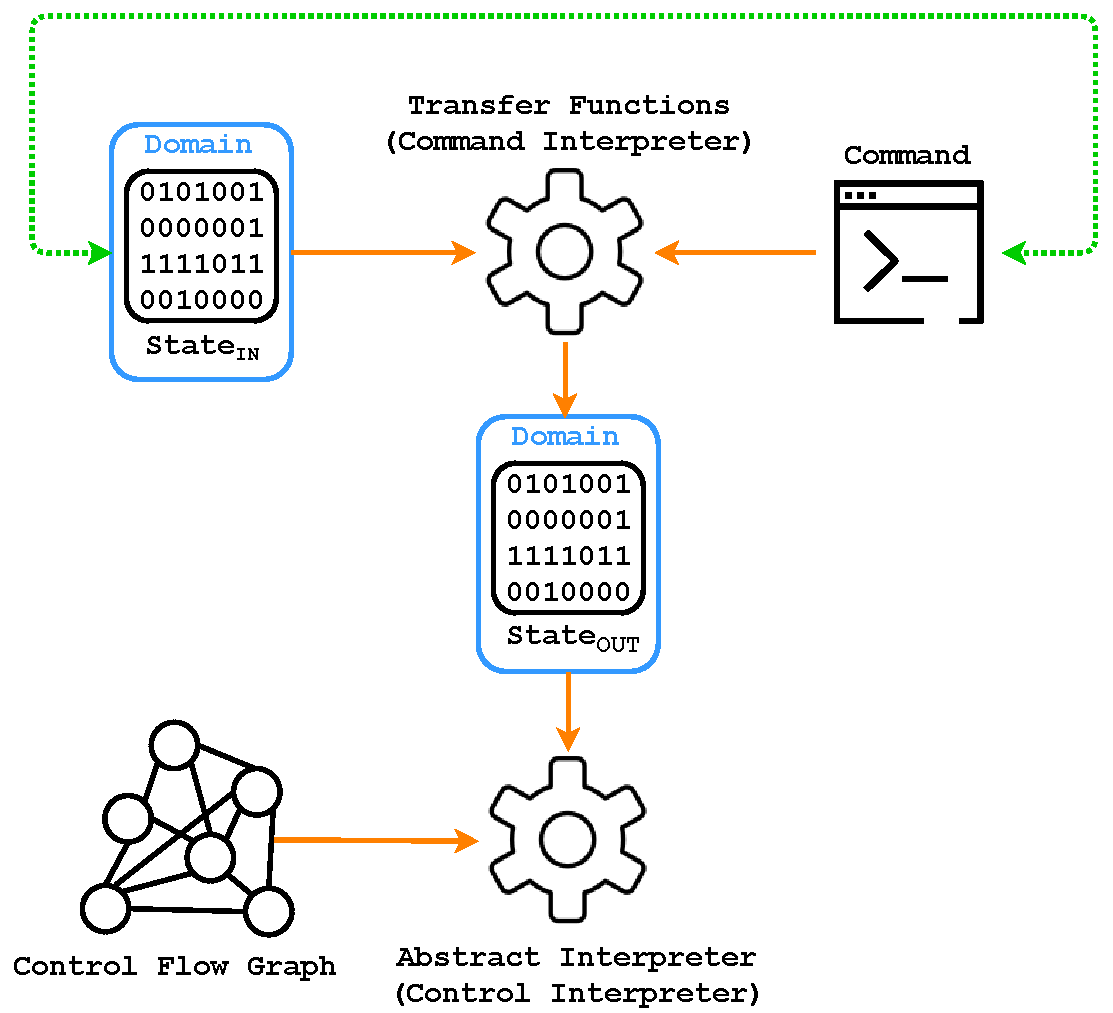
\includegraphics[width=.65 \linewidth]{infer_analysis.pdf}
    \caption{%
        Facebook Infer's abstract interpretation
        process~\cite{inferAISlides, projectPracticeMarcin2018}
    }
    \label{fig:inferAnalysis}
\end{figure}


\section{Contracts for Concurrency}
\label{sec:contracts}

This section introduces the concept of \emph{contracts for concurrency}
described in~\cite{contracts2015, contracts2017}. Parts of this section are
taken from the paper~\cite{excel2019FBInfer}. Listings in this section are
pieces of programs written in ANSI~C.

Respecting the \emph{protocol} of a~software module\,---\,defines
which \emph{sequences of functions} are legal to invoke\,---\,is one of the
requirements for the correct behaviour of the module. For example, a~module
that deals with a~file system typically requires that a~programmer using
this module should call function \texttt{open} at first, followed by an
optional number of functions \texttt{read} and \texttt{write}, and at last,
call function \texttt{close}. A~program utilising such a~module that does
not follow this protocol is erroneous. The methodology of \emph{design by
contract} (described in~\cite{contract}) requires programs to meet
such well-defined behaviours.~\cite{contracts2015}

In \emph{concurrent programs}, contracts for concurrency allow 
one\,---\,in the simplest case\,---\,to specify \emph{sequences of 
functions} that are needed to be \emph{executed atomically} in order to 
avoid \emph{atomicity violations}. In general, contracts for concurrency 
specify sets of sequences of calls that are called \emph{spoilers} and sets 
of sequences of calls that are called \emph{targets}, and it is then 
required that no target overlaps fully with any spoiler. Such contracts may 
be manually specified by a~developer or they may be automatically generated 
by a~program (analyser). These contracts can be used to verify the 
correctness of programs as well as they can serve as helpful documentation.

Section~\ref{sec:basicContracts} defines the notion of \emph{basic contracts
for concurrency}. Further, Section~\ref{sec:paramContracts} defines
contracts extended to consider the \emph{data flow} between functions 
(where a~sequence of function calls must be atomic only if they handle the
same data). The above mentioned more general contracts for concurrency with
spoilers and targets, which essentially extend the basic contracts with
some \emph{contextual information}, are not presented here in detail 
(they are explained in the paper~\cite{contracts2017}). The reason is that
the proposed analyser\,---\,\emph{Atomer}\,---\,so far concentrates on the 
basic contracts.


\subsection{Basic Contracts}
\label{sec:basicContracts}

In~\cite{contracts2017, contracts2015}, a~\emph{basic contract} is
formally defined as follows. Let~$ \Sigma_\mathbb{M} $~be a~set of all
function names of a~software module. A~contract is
a~set~$ \mathbb{R} $~of \emph{clauses} where each clause
$ \varrho\ \in \mathbb{R} $ is a~\emph{star-free regular
expression}\footnote{\textbf{Star-free regular expressions} are
regular expressions using only the \emph{concatenation operators}
and the \emph{alternative operators} ($ | $), without the
\emph{Kleene star operator} ($ * $).} over~$ \Sigma_\mathbb{M} $.
A~\emph{contract violation} occurs if any of the sequences expressed by
the contract clauses are interleaved with the execution of functions
from~$ \Sigma_\mathbb{M} $, in other words, each sequence specified by
any clause~$ \varrho $~must be executed atomically, otherwise, there
is a~violation of the contract. The number of sequences defined by
a~contract is finite since the contract is the union of
\emph{star-free languages}.

\begin{example}
    Consider the following example from~\cite{contracts2017, contracts2015}. 
    Assume that there is a~module implementing a~resizable array 
    implementing the following interface functions:
    \begin{enumerate}[label={$ f_{\arabic*} $:}]
        \tt

        \item
            \textcolor{bluekeywords}{void} add(%
                \textcolor{bluekeywords}{char} *array,
                \textcolor{bluekeywords}{char} element%
            )

        \item
            \textcolor{bluekeywords}{bool} contains(%
                \textcolor{bluekeywords}{char} *array,
                \textcolor{bluekeywords}{char} element%
            )

        \item
            \textcolor{bluekeywords}{int} index\_of(%
                \textcolor{bluekeywords}{char} *array,
                \textcolor{bluekeywords}{char} element%
            )

        \item
            \textcolor{bluekeywords}{char} get(%
                \textcolor{bluekeywords}{char} *array,
                \textcolor{bluekeywords}{int} index%
            )

        \item
            \textcolor{bluekeywords}{void} set(%
                \textcolor{bluekeywords}{char} *array,
                \textcolor{bluekeywords}{int} index,
                \textcolor{bluekeywords}{char} element%
            )

        \item
            \textcolor{bluekeywords}{void} remove(%
                \textcolor{bluekeywords}{char} *array,
                \textcolor{bluekeywords}{int} index%
            )

        \item
            \textcolor{bluekeywords}{int} size(%
                \textcolor{bluekeywords}{char} *array%
            )
    \end{enumerate}
    \newpage
    The module's contract contains the following clauses:
    \begin{enumerate}[label={$ (\varrho_{\arabic*}) $}]
        \item
            \texttt{contains index\_of}
            \begin{itemize}[label=]
                \item
                    The execution of \texttt{contains} followed by the execution
                    of \texttt{index\_of} should be atomic. Otherwise,
                    the program may fail to get the index, because after
                    verification of the presence of an element in an array, it
                    can be removed by some \emph{concurrently running process}.
            \end{itemize}

        \item
            \texttt{index\_of (get | set | remove)}
            \begin{itemize}[label=]
                \item
                    The execution of \texttt{index\_of} followed by the
                    execution of \texttt{get}, \texttt{set}, or 
                    \texttt{remove} should be atomic. Otherwise, the received
                    index may be outdated when it is applied to the address
                    of an element, because a~concurrent modification of an 
                    array may shift the position of the element.
            \end{itemize}

        \item
            \texttt{size (get | set | remove)}
            \begin{itemize}[label=]
                \item
                    The execution of \texttt{size} followed by the execution of
                    \texttt{get}, \texttt{set}, or \texttt{remove} should be
                    atomic. Otherwise, the size of an array may be void when
                    accessing an array, because of a~concurrent change of the
                    array. This can be an issue since a~given index is not in
                    a~valid range anymore (e.g., testing \texttt{index < size}).
            \end{itemize}

        \item
            \texttt{add (get | index\_of)}
            \begin{itemize}[label=]
                \item
                    The execution of \texttt{add} followed by the execution of
                    \texttt{get} or \texttt{index\_of} should be atomic.
                    Otherwise, the added element needs no longer exist or its
                    position in an array can be changed, when the program
                    tries to obtain information about it.
            \end{itemize}
    \end{enumerate}
\end{example}


\subsection{Contracts with Parameters}
\label{sec:paramContracts}

The above definition of basic contracts is quite limited in some 
circumstances and can consider valid programs as erroneous (reports 
\emph{false alarms}). Hence, in this section, there is defined an extension 
of basic contracts\,---\,\emph{contracts with parameters}\,---\,which takes 
into consideration the data flow within function calls.

\begin{example}
    Consider the following example from~\cite{contracts2017, contracts2015}, 
    given Listing~\ref{list:contractsReplace}. There is a~function
    \texttt{replace} that replaces item~\texttt{a}~in an array by 
    item~\texttt{b}. The implementation of this function comprises two 
    atomicity violations:
    \begin{enumerate}[label={(\roman*)}]
        \item
            when \texttt{index\_of} is invoked, item~\texttt{a}~does not need to
            be in the array anymore;

        \item
            the acquired index can be obsolete when \texttt{set} is invoked.
    \end{enumerate}
    A~basic contract could cover this scenario by the clause~$ \varrho_5 $:
    $$ (\varrho_5)\ \text{\texttt{contains index\_of set}} $$
    Nevertheless, this definition is too restrictive because the functions
    are required to be executed atomically only if \texttt{contains} and
    \texttt{index\_of} have the same arguments \texttt{array} and
    \texttt{element}, \texttt{index\_of} and \texttt{set} have the same 
    argument \texttt{array}, and the returned value of \texttt{index\_of} is
    used as the argument \texttt{index} of the function \texttt{set}.
\end{example}

\begin{lstlisting}[
    style=c, label={list:contractsReplace}, float=hbt,
    caption={%
        An example of an atomicity violation with data
        dependencies~\cite{contracts2017}
    }
]
void replace(char *array, char a, char b)
{
    if (contains(array, a))
    {
        int index = index_of(array, a);
        set(array, index, b);
    }
}
\end{lstlisting}

In order to respect function call \emph{parameters} and \emph{return values}
of functions in contracts, the basic contracts are extended by
dependencies among functions in~\cite{contracts2017, contracts2015}
as follows. Function call parameters and return values are expressed as
\emph{meta-variables}. Further, if a~contract should be required to be
observed exclusively if the same object emerges as an argument or as the 
return value of multiple calls in a~given call sequence, it may be denoted 
by using the same meta-variable at the position of all these occurrences of
parameters and return values.

Clause~$ \varrho_5 $~can be extended as follows (repeated application of
meta-variables \texttt{X/Y/Z} requiring the same objects
\texttt{o\textsubscript{1}/o\textsubscript{2}/o\textsubscript{3}} to be used
at the positions of \texttt{X/Y/Z}):
$$
    (\varrho'_5)\ \text{\texttt{%
        contains(X,Y) Z=index\_of(X,Y) set(X,Z,\_)
    }}
$$
The underscore indicates a~\emph{free meta-variable} that does not restrict
the contract clause.

With the extension described above, it is possible to extend the contract
from Section~\ref{sec:basicContracts} as follows:
\begin{enumerate}[label={$ (\varrho'_{\arabic*}) $}]
    \tt

    \item contains(X,Y) index\_of(X,Y)
    \item Y=index\_of(X,\_) (get(X,Y) | set(X,Y,\_) | remove(X,Y))
\end{enumerate}



%===============================================================================
\chapter{Atomicity Violations Detector}
\label{chap:proposal}

In this chapter, there are described principles behind the static analyser
\textbf{Atomer} that have been proposed as a~module of \emph{Facebook
Infer} (introduced in Section~\ref{sec:fbinfer}) for detection of
\emph{atomicity violations}. In particular, the Atomer concentrates on 
checking \emph{atomicity of execution of certain sequences of function 
calls} that is often required for a~correct functioning of concurrent 
programs. The proposed principle is based on the assumption that sequences
executed \emph{atomically once} should probably be executed \emph{always
atomically}. The chapter also discusses already existing solutions in this
area.

At first, Section~\ref{sec:relWork} deals with
existing approaches and tools for finding atomicity violations, their
advantages, disadvantages, features, availability, and so on. Then,
the proposed analysis algorithm that is behind Atomer is introduced in
Section~\ref{sec:design}. Parts of this chapter are taken from the
paper~\cite{excel2019FBInfer}. Listings in this chapter are pieces of 
exemplary programs written in ANSI~C (assuming \emph{PThread} locks and the
existence of an initialised global variable \texttt{lock} of a~type
\texttt{pthread\_mutex\_t}).


\section{Related Work}
\label{sec:relWork}

The proposed solution is slightly inspired by ideas from~\cite{contracts2017,
contracts2015}. In these papers, there is described a~proposal and 
implementation of a~\emph{static validation} for finding some forms of
\emph{atomicity violations}, which is based on \emph{grammars} and
\emph{parsing trees}. In the paper~\cite{contracts2017}, there is also 
described and implemented a~\emph{dynamic} approach for the validation. The
authors of~\cite{contracts2017, contracts2015} implemented a~stand-alone
prototype tool\footnote{\textbf{Gluon}\,---\,a~tool for static verification of
\emph{contracts for concurrency} (see Section~\ref{sec:contracts}) in Java
programs\,---\,\url{https://github.com/trxsys/gluon}.} for analysing programs
written in Java. It led to some promising experimental results but the
\emph{scalability} of the tool was still limited. Moreover, the tool
from~\cite{contracts2017, contracts2015} is no more developed. This
fact inspired the decision that eventually led to this thesis, namely, to
get inspired by the ideas of~\cite{contracts2017, contracts2015}, but
reimplement them in \emph{Facebook Infer} redesigning it in accordance 
with the principles of Facebook Infer (described in 
Section~\ref{sec:fbinfer}), which should make the resulting tool more 
scalable. In the end, however, due to adapting the analysis for the context 
of Facebook Infer, the implementation of the analysis within this thesis is
significantly different from~\cite{contracts2017, contracts2015}, as it is
presented in Chapter~\ref{chap:implement}. Furthermore,
unlike~\cite{contracts2017, contracts2015}, the implementation aims at 
programs written in the C/C++ languages using \emph{POSIX Thread (PThread)} 
locks for \emph{synchronisation of concurrent threads}.

In Facebook Infer, there is already implemented an analysis called
\emph{Lock Consistency Violation}\footnote{\textbf{Lock Consistency
Violation}\,---\,atomicity violations analysis in Facebook
Infer\,---\,\url{https://fbinfer.com/docs/%
checkers-bug-types.html\#LOCK_CONSISTENCY_VIOLATION}.}. It is a~part of
\emph{RacerD}~\cite{racerD, racerDOnline, staticRaceDetectorTruePositive}. 
This analysis finds atomicity violations for writes/reads on single 
variables that are required to be executed atomically. Atomer is different, 
it finds atomicity violations for \emph{sequences of functions} that are 
required to be executed atomically, i.e., it checks whether \emph{contracts 
for concurrency} (see Section~\ref{sec:contracts}) hold. Moreover, it is 
trying to automatically find out which of the sequence should indeed 
be executed atomically (hence, to \emph{automatically derive the
contracts}).


\section{Analysis and Design}
\label{sec:design}

As it has been already said, the proposal of the analyser is based on 
the concept of \emph{contracts for concurrency} described in
Section~\ref{sec:contracts}. In particular, the proposal considers 
\emph{basic contracts} described in Section~\ref{sec:basicContracts}.
Neither the contracts extended to \emph{spoilers} and \emph{targets} 
nor contracts extended by \emph{parameters} (see
Section~\ref{sec:paramContracts}) are so far taken into account.

In general, basic contracts for concurrency allow one to define
\emph{sequences of functions} that are required to be \emph{executed
atomically}, as it is explained in more detail in Section~\ref{sec:contracts}.
Atomer is able to automatically derive candidates for such contracts, and
then to verify whether the contracts are fulfilled. Both of these steps
are done statically. The proposed analysis is divided into two parts
(\emph{phases of the analysis}):
\begin{enumerate}[label={\textbf{Phase \arabic*}:}, leftmargin=6em]
    \item
        Detection of (likely) \emph{atomic sequences}, which is described 
        in Section~\ref{sec:designPhase1}.

    \item
        Detection of \emph{atomicity violations} (violations of the atomic
        sequences), which is described in Section~\ref{sec:designPhase2}.
\end{enumerate}
These phases of the analysis and its workflow are illustrated in
Figure~\ref{fig:analyserPhases}.

\begin{figure}[hbt]
    \centering
    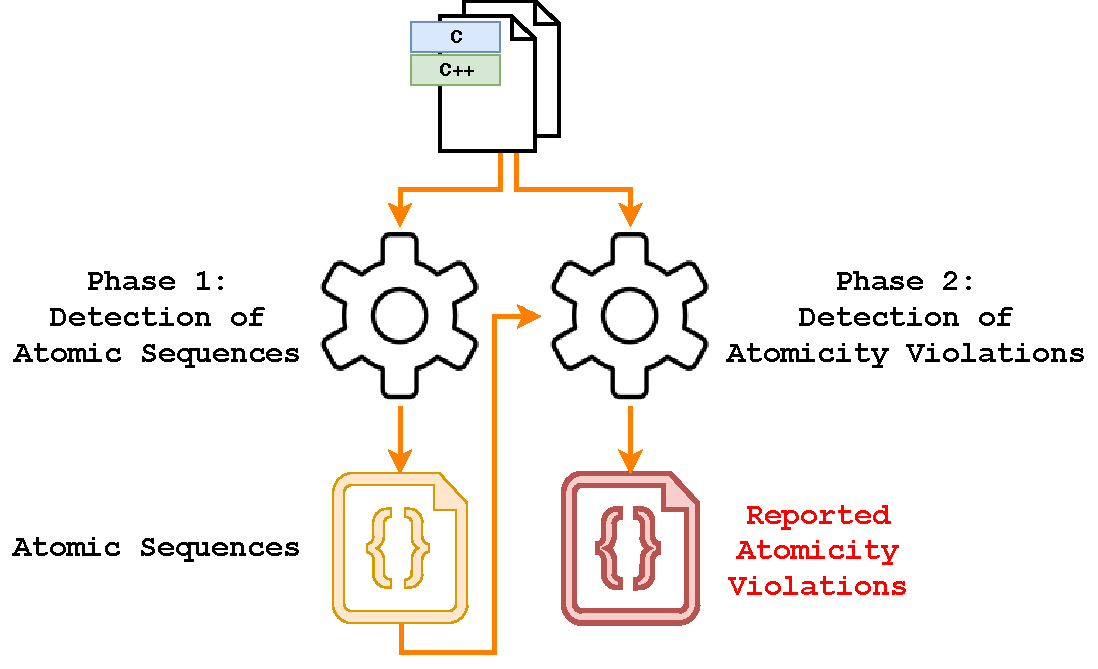
\includegraphics[width=.75 \linewidth]{analyser_proposal.pdf}
    \caption{Phases of the proposed analyser}
    \label{fig:analyserPhases}
\end{figure}

This section describes the proposal in general. The concrete types
of the \emph{abstract states} and the \emph{summaries}, along with the
implementation of all the necessary \emph{abstract interpretation 
operators} are described in Chapter~\ref{chap:implement}. But
in general, the abstract states of both phases of the analysis
are proposed as sets. So, in fact, the \emph{ordering} operator
is implemented using testing for a~\emph{subset}, the \emph{join}
operator is implemented as a~\emph{union}, and the \emph{widening}
operator is implemented using the join operator. Implementation of the
\emph{abstract domain} is detailed in Chapter~\ref{chap:implement}.

Function summaries are in below sections reduced to the output parts only.
The input parts of summaries are in case of the proposed analysis always 
empty, because, so far, it is not necessary to have any \emph{preconditions}
for analysed functions.


\newpage
\subsection{Phase 1: Detection of Atomic Sequences}
\label{sec:designPhase1}

Before the detection of \emph{atomicity violations} may begin, it is 
required to have contracts introduced in Section~\ref{sec:contracts}.
\textbf{Phase 1} of Atomer is able to produce such contracts, i.e., 
it detects \emph{sequences of functions} that should be \emph{executed
atomically}. Intuitively, the detection is based on looking for sequences 
of functions that are executed atomically on some path through
a~program. The assumption is that if it is once needed to execute
a~sequence atomically, it should probably be always executed atomically.

To be able to describe the analysis, it is first needed to introduce
a~notion of a~\emph{reduced sequence} of function calls. Such a~sequence
denotes a~sequence in which the first appearance of each function is 
recorded only. The reason is to ensure \emph{finiteness} of the sequences 
derived by the analysis and hence termination of the analysis. The detection 
of sequences of calls to be executed atomically is based on analysing all 
paths through the CFG of a~function and generating all pairs~\textbf{(A,~B)} 
of sets of function calls such that: Here, \textbf{A}~is a~reduced
sequence of function calls that appear between the beginning of the function
being analysed and the first lock, between an unlock and a~subsequent lock, 
or between an unlock and the end of the function being analysed. \textbf{B}~is
a~reduced sequence of function calls that follow the calls from~\textbf{A}~and
that appear between a~lock and an unlock (or between a~lock and the end of 
the function being analysed).

It would be more precise to generate longer sequences of 
the type~\textbf{A\textsubscript{1}B\textsubscript{1}A\textsubscript{2}%
B\textsubscript{2}\ldots}, instead of the sets of the 
sequences~\textbf{(A,~B)}. But it would be more difficult to ensure the
finiteness of the above longer sequences and the finiteness of sets of 
these sequences. Moreover, there would be a~significantly larger 
\emph{state explosion problem}. So, the proposed representation of the 
sets of pairs of sequences has been chosen as a~compromise between 
accuracy and efficiency. But the experiments (described in 
Chapter~\ref{chap:exp}) show that for appropriate \emph{scalability} will 
be (in future) needed more pronounced abstraction.

\begin{example}
    For explanation of the computation of the sets of the 
    sequences~\textbf{(A,~B)}, assume that a~state of the analysis of 
    the program~$ P $~is the following sequence of function calls:
    \texttt{f1}~\texttt{f2}; and a~state of the analysis of the 
    program~$ P' $~is the following sequence of function calls:
    \texttt{f1}~\texttt{f2}~(\texttt{g1}~\texttt{g2}. The parentheses 
    are used to indicate an \emph{atomic sequence} (closing parenthesis is 
    missing in the second case, which means that the program state is 
    currently inside an \emph{atomic block}). The computed set for the
    program~$ P $~is $ P_s = $~\{[\texttt{f1}~\texttt{f2};~%
    \textvisiblespace]\}, and for the program~$ P' $, it is $ P'_s = $~%
    \{[\texttt{f1}~\texttt{f2};~\texttt{g1}~\texttt{g2}]\}. Now, if the next
    instruction is a~call of the function~\texttt{x}, in the case of the
    program~$ P $, the call will be added to the~\textbf{A}~sequence, and in 
    the case of the program~$ P' $, the call will be added to
    the~\textbf{B}~sequence as follows: $ P_s = $~\{[\texttt{f1}~%
    \texttt{f2}~\texttt{x};~\textvisiblespace]\}, $ P'_s = $~%
    \{[\texttt{f1}~\texttt{f2};~\texttt{g1}~\texttt{g2}~\texttt{x}]\}.
    Subsequently, if the next step in the program~$ P $~is a~lock call,
    the next function calls will be added to the~\textbf{B}~sequence of the
    set~$ P_s $. And if the next step in the program~$ P' $~is an unlock 
    call, it will be created a~new element of the set~$ P'_s $ and the
    next function call will be added to the~\textbf{A}~sequence of this set.
    Finally, if the function~\texttt{y}~is called, the resulting sets
    will look like follows: $ P_s = $~\{[\texttt{f1}~\texttt{f2}~%
    \texttt{x};~\texttt{y}]\}, $ P'_s = $~\{[\texttt{f1}~\texttt{f2};~%
    \texttt{g1}~\texttt{g2}~\texttt{x}],~[\texttt{y};~\textvisiblespace\}.
\end{example}

The \emph{summary} of a~function then consists of:
\begin{enumerate}[label={(\roman*)}]
    \item
        The set of all the~\textbf{B}~sequences that appear on program
        paths through the function.

    \item
        The \emph{concatenation} of all
        the~\textbf{A}~and \textbf{B}~sequences with removed duplicates 
        of function calls. In particular, assume that there is the
        following computed set of the sequences~\textbf{(A,~B)}:~%
        $ \{(A_1; B_1), (A_2; B_2), \ldots, (A_n; B_n)\} $, then
        the result of the concatenation is the sequence~$ A_1{\cdot}B_1%
        {\cdot}A_2{\cdot}B_2{\cdot} \ldots {\cdot}A_n{\cdot}B_n $.
        Intuitively, in this component of the summary, it is gathered
        occurrences of all called functions within an analysed function,
        which is obtained by concatenation of all
        the~\textbf{A}~and \textbf{B}~sequences.
\end{enumerate}
The latter is recorded for the purpose of analysing functions higher in the
\emph{call hierarchy} since locks/unlocks can appear in such
a~\emph{higher-level function}.

\begin{example}
    For instance, the analysis of the function~\texttt{g}~from
    Listing~\ref{list:analyserPhase1} produces the following sequences:
    $$
        \overbrace{%
            \text{\texttt{f1}~\sout{\texttt{f1}}}
        }^\text{\textbf{A\textsubscript{1}}}
        \overbrace{%
            (\text{\texttt{f1}~\sout{\texttt{f1}}~\texttt{f2}})
        }^\text{\textbf{B\textsubscript{1}}} |
        \overbrace{%
            \text{\texttt{f1}~\sout{\texttt{f1}}}
        }^\text{\textbf{A\textsubscript{2}}}
        \overbrace{%
            (\text{\texttt{f1}~\texttt{f3}})
        }^\text{\textbf{B\textsubscript{2}}} |
        \overbrace{%
            \text{\sout{\texttt{f1}}}
        }^\text{\sout{\textbf{A\textsubscript{3}}}}
        \overbrace{%
            (\text{\sout{\texttt{f1}~\texttt{f3}~\texttt{f3}}})
        }^\text{\sout{\textbf{B\textsubscript{3}}}}
    $$
    The functions~\texttt{f1}, \texttt{f2}, \texttt{f3} are not deeper
    analysed because it is assumed that these functions are leaf nodes
    of the \emph{call graph}.
    The strikethrough of the functions~\texttt{f1} and \texttt{f3} denotes
    the removal of already recorded function calls in
    the~\textbf{A}~and \textbf{B}~sequences. The strikethrough of the
    entire sequence~\texttt{f1}~(\texttt{f1}~\texttt{f3}~\texttt{f3})
    means discarding sequences already seen before. The derived summary
    components for the function~\texttt{g}~are then as follows:
    \begin{enumerate}[label={(\roman*)}]
        \item
           \{(\texttt{f1}~\texttt{f2}),~(\texttt{f1}~\texttt{f3})\}, i.e.,
           \textbf{B\textsubscript{1}}~and \textbf{B\textsubscript{2}};

        \item
            \texttt{f1}~\texttt{f2}~\texttt{f3}, i.e.,
            the concatenation of~\textbf{A\textsubscript{1}},
            \textbf{B\textsubscript{1}}, \textbf{A\textsubscript{2}},
            and \textbf{B\textsubscript{2}} from which duplicate
            function calls were removed.

    \end{enumerate}
\end{example}

\begin{lstlisting}[
    style=c, label={list:analyserPhase1}, float=hbt,
    caption={%
        A~code snippet used for illustration of the derivation of
        sequences of functions called atomically
    }
]
void g(void)
{
    f1(); f1();

    <@\textcolor{red}{pthread\_mutex\_lock}@>(&lock);
    f1(); f1(); f2();
    <@\textcolor{red}{pthread\_mutex\_unlock}@>(&lock);

    f1(); f1();

    <@\textcolor{red}{pthread\_mutex\_lock}@>(&lock);
    f1(); f3();
    <@\textcolor{red}{pthread\_mutex\_unlock}@>(&lock);

    f1();

    <@\textcolor{red}{pthread\_mutex\_lock}@>(&lock);
    f1(); f3(); f3();
    <@\textcolor{red}{pthread\_mutex\_unlock}@>(&lock);
}
\end{lstlisting}

Further, it is demonstrated how the results of the analysis of \emph{nested
functions} are used during the detection of atomic sequences. The
result of the analysis of a~nested function is used as follows. When
calling an already analysed function, one plugs the sequence from the
second component of its summary into the
current~\textbf{A}~or~\textbf{B}~sequence. In particular, assume 
that~$ (A, B) $~is the current pair of sequences of the actual state of 
the analysis. Subsequently, it is called the function~\texttt{f}~with
\emph{non-empty summary}, where~$ S $~is the second component of its 
summary. If the current state of an analysed function is inside an
atomic block, the result of this step of the analysis will 
be~$ (A, B\cdot\mathtt{f}{\cdot}S) $, otherwise, the result will 
be~$ (A\cdot\mathtt{f}{\cdot}S, B) $. In such cases where a~summary
is empty, i.e., an analysed function is a~leaf node of the call
graph, it is appended just the function name to the current pair of
sequences of the actual state of the analysis.

\begin{example}
    This example shows how the function~\texttt{h}~from
    Listing~\ref{list:analyserPhase1Nested} would be analysed using the
    result of the analysis of the function~\texttt{g}~from
    Listing~\ref{list:analyserPhase1}. So the analysis of the
    function~\texttt{h}~produces the following sequence:
    $$
        \text{%
            \texttt{f1}~\texttt{g}~\sout{\texttt{f1}}~\texttt{f2}~\texttt{f3}
        }
        (\text{%
            \texttt{g}~\texttt{f1}~\texttt{f2}~\texttt{f3}%
        })
    $$
    The derived summary components for the function~\texttt{h}~are then as
    follows:
    \begin{enumerate}[label={(\roman*)}]
        \item
            \{(\texttt{g}~\texttt{f1}~\texttt{f2}~\texttt{f3})\};

        \item
            \texttt{f1}~\texttt{g}~\texttt{f2}~\texttt{f3}.
    \end{enumerate}
\end{example}

\begin{lstlisting}[
    style=c, label={list:analyserPhase1Nested}, float=hbt,
    caption={%
        A~code snippet used for illustration of the derivation of
        sequences of functions called atomically with a~nested function
        call (function~\texttt{g} is defined in
        Listing~\ref{list:analyserPhase1})
    }
]
void h(void)
{
    f1(); g();

    <@\textcolor{red}{pthread\_mutex\_lock}@>(&lock);
    g();
    <@\textcolor{red}{pthread\_mutex\_unlock}@>(&lock);
}
\end{lstlisting}

\newpage
\subsubsection{Cases Where Lock/Unlock Calls Are Not Paired in a~Function}

For treating cases where lock/unlock calls are \emph{not paired} in
a~function\,---\,as demonstrated
Listing~\ref{list:analyserPhase1NotPairedLock}\,---\,two solutions
have been proposed:
\begin{enumerate}
    \item
        At the end of a~function, everything is unlocked, i.e., one
        virtually appends an unlock to the end of the function if it 
        is necessary. Then for the function~\texttt{x}~from
        Listing~\ref{list:analyserPhase1NotPairedLock}, the first component
        of its summary (i.e., atomic sequences) would be \{(\texttt{a})\}.
        Subsequently, all unlock calls not preceded by a~lock are
        ignored. So the first component of a~summary of the
        function~\texttt{y}~from
        Listing~\ref{list:analyserPhase1NotPairedLock} would be the empty 
        set.

    \item
        Addition of two further items to the summaries:
        \begin{enumerate}[label={(\alph*)}]
            \item
                function calls missing an unlock call,

            \item
                function calls missing a~lock call.
        \end{enumerate}
        For the example from Listing~\ref{list:analyserPhase1NotPairedLock},
        this would give:
        \begin{itemize}
            \item
                for~\texttt{x}:~\{(\texttt{f1}\},

            \item
                for~\texttt{y}:~\{\texttt{f2})\}.
        \end{itemize}
        The above sequences would have to be glued to the sequences
        captured higher in the call hierarchy. Calls of the
        functions~\texttt{f1} and \texttt{f2} will also appear in
        the second component of the function summaries (i.e., the sequences
        of all functions called).
\end{enumerate}

\begin{lstlisting}[
    style=c, label={list:analyserPhase1NotPairedLock}, float=hbt,
    caption={%
        A~code snippet used for illustration of treating cases where
        lock/unlock calls are not paired in a~function
    }
]
void x(void)
{
    <@\textcolor{red}{pthread\_mutex\_lock}@>(&lock);
    f1();
}

void y(void)
{
    f2();
    <@\textcolor{red}{pthread\_mutex\_unlock}@>(&lock);
}

void main(void)
{
    x(); y();
}
\end{lstlisting}

In the end, the first approach of treating such cases described above has
been chosen. The reason is that it is much easier for implementation.
However, in future, the analysis can be improved by implementing the second
approach.

\newpage
\subsubsection{%
    Summary of the Detection of Atomic Sequences and Future Work
}

The above detection of atomic sequences has been implemented, as it is
described in Section~\ref{sec:implementPhase1}. Furthermore, it has
been successfully verified on a~set of sample programs created for
testing purposes. The verification is presented in Chapter~\ref{chap:exp} and 
in Section~\ref{sec:expResPhase1}. The derived sequences of calls assumed to
execute atomically, i.e., the \textbf{B}~sequences, from the summaries
of all analysed functions are stored into a~file, which is used during
\textbf{Phase~2}, described below in Section~\ref{sec:designPhase2}.
There are some possibilities for further extending and improving
\textbf{Phase~1}, e.g., working with \emph{nested locks}; distinguishing
the \emph{different locks} used (currently, it is not distinguished
between the locks at all); considering \emph{contracts for concurrency with
parameters} defined in Section~\ref{sec:paramContracts} or other extensions
of contracts for concurrency discussed in Section~\ref{sec:contracts}; or
extending the detection for \emph{other types of locks} for synchronisation
of concurrent threads/processes. On the other hand, to further enhance the
\emph{scalability}, it seems promising to replace working with the
\textbf{A}~and~\textbf{B}~sequences by working with sets of calls: sacrificing
some precision but gaining the speed.


\subsection{Phase 2: Detection of Atomicity Violations}
\label{sec:designPhase2}

In the second phase of the analysis, i.e., when \emph{detecting
violations} of the atomic sequences obtained from \textbf{Phase~1}, the 
analysis looks for pairs of functions that should be called atomically 
(or just for single functions if there is only one function call in an 
atomic sequence) while this is not the case on some path through the CFG.
The pairs of a~function whose calls are to be checked for atomicity are
obtained as follows: For each function in a~given program, it is taken
the first component of its \emph{summary}~$ \{B_1, B_2, \ldots, B_l\} $
and it is taken every pair of functions~\texttt{f1}~\texttt{f2}~that
appears as a~\emph{substring} in some of the~$ B_i $~sequences, 
i.e.,~$ B_i = w_1\mathtt{f1f2}w_2 $ for some sequences~$ w_1 $~and~$ w_2 $.
Moreover, if some~$ B_i $ consists of a~single function, it is checked
that this function is always called under a~lock. The implementation of 
an algorithm for this detection is described in
Section~\ref{sec:implementPhase2}, particularly, in
Algorithm~\ref{alg:phase2UpdateAstateFunCall}.

\begin{example}
    For example, assume that the result of the first phase is the following
    set of functions called atomically (all the atomic sequences from
    all functions in an analysed program):
    $$
        \text{%
            \{(\texttt{f1}~\texttt{f2}~\texttt{f3}),
            (\texttt{f1}~\texttt{f3}~\texttt{f4})\}
        }
    $$
    Then the analysis will look
    for the following pairs of functions that are not called atomically:
    \begin{itemize}
        \item \texttt{f1}~\texttt{f2}
        \item \texttt{f2}~\texttt{f3}
        \item \texttt{f1}~\texttt{f3}
        \item \texttt{f3}~\texttt{f4}
    \end{itemize}
\end{example}

The analysis of functions with nested function calls and cases where 
lock/unlock calls are not paired in a~function are handled analogically
as in \textbf{Phase~1}. For detailed examples see verification experiments 
in Section~\ref{sec:expResPhase2}.

\begin{example}
    For a~demonstration of the detection of an atomicity violation, assume
    the functions~\texttt{a}~and~\texttt{b}~from
    Listing~\ref{list:analyserPhase2}. The set of atomic sequences of the
    function~\texttt{a}~is \{(\texttt{f2}~\texttt{f3})\}. In the function
    \texttt{b}, an atomicity violation is detected because the
    functions~\texttt{f2} and \texttt{f3} are not called atomically (under
    a~lock).
\end{example}

\begin{lstlisting}[
    style=c, label={list:analyserPhase2}, float=hbt,
    caption={Example of an atomicity violation}
]
void a(void)
{
    f1();

    <@\textcolor{red}{pthread\_mutex\_lock}@>(&lock);
    f2(); f3();
    <@\textcolor{red}{pthread\_mutex\_unlock}@>(&lock);

    f4();
}

void b(void)
{
    f1(); f2(); f3(); f4();
}
\end{lstlisting}

\newpage
\subsubsection{%
    Summary of the Detection of Atomicity Violations and Future Work
}

Like in the first phase of the analysis, \textbf{Phase~2} has been
implemented, as it is described in Section~\ref{sec:implementPhase2}.
The implementation has been also successfully verified on a~set of 
sample purposeful programs as discussed in Chapter~\ref{chap:exp} and in
Section~\ref{sec:expResPhase2}. \textbf{Phase~2} also has the potential for 
further enhancing. It is possible to extend this phase with all the 
improvements discussed in Section~\ref{sec:designPhase1}. The next idea 
is to consider atomic sequences from the first phase only if they appear 
in an \emph{atomic block} more than, e.g., three times. It would strengthen 
the certainty that such a~sequence should be called atomically.



%===============================================================================
\chapter{Implementation}
\label{chap:implement}

This chapter describes the implementation of the \emph{static 
analyser}\,---\,\emph{Atomer}\,---\,proposed in Chapter~\ref{chap:proposal}. 
The analyser is implemented as a~module of \emph{Facebook Infer} introduced 
in Section~\ref{sec:fbinfer}. The implementation is demonstrated using
algorithms in \emph{pseudocode} and using listings with codes written 
in \emph{OCaml}, which is an implementation language of Facebook Infer.
Sections~\ref{sec:implementPhase1} and~\ref{sec:implementPhase2}
describes the implementation of the \emph{detection of atomic sequences} 
defined in Section~\ref{sec:designPhase1} and an implementation of the
\emph{detection of atomicity violations} defined in
Section~\ref{sec:designPhase2}, respectively.

The implementation of the analyser can be found publicly on
GitHub\footnote{\textbf{The implementation of the analyser} in a~GitHub
repository, which is a~\emph{fork} of the official repository of Facebook
Infer, in a~branch
\texttt{atomicity}\,--\,\url{https://github.com/harmim/infer/tree/atomicity}.}.
The implementation is done in OCaml and it exploits both \emph{functional}
and \emph{imperative} paradigm. Facebook Infer supports analysis of
programs written in Java, C, C++, and Objective-C. However, the implementation
aims at programs written in the C/C++ languages using \emph{POSIX Thread
(PThread)} locks, which is a~\emph{low-level} mechanism for
\emph{synchronisation of concurrent threads}. So, the analyser understands 
the \texttt{pthread\_mutex\_lock} as the lock function and the
\texttt{pthread\_mutex\_unlock} as the unlock function. It is also possible 
to run the analysis on programs written in Java or Objective-C languages but
the result of the analysis would be likely wrong since these languages use
a~different mechanism for synchronisation.

\textbf{Phase~1}, i.e., the detection of atomic sequences and \textbf{Phase~2},
i.e., the detection of atomicity violations are implemented as separate
analysers in Facebook Infer. The output of the first phase is the input of
the second phase (as shown in Figure~\ref{fig:analyserPhases}). Both of
these analysers are registered as modules of Facebook Infer in a~file
\hyptt{infer/src/checkers/registerCheckers.ml}. These analyses run only
if a~particular command line argument of Facebook Infer is specified.
Implementations of individual phases are discussed below
(Section~\ref{sec:implementPhase1} and Section~\ref{sec:implementPhase2}).

In order to make the analysis \emph{interprocedural}, it is necessary to
define a~type of function \emph{summaries} for each phase.
The types of summaries are defined in \emph{abstract domains} of
each phase. However, the summaries are stored and accessed using
the module \texttt{Payloads} (called as the \emph{summary payload}). 
Fields of the payload that refer to the summaries of the analysis are 
defined in a~file \texttt{infer/src/backend/Payloads.ml[i]}.

For both phases of the analysis, the analyser is implemented as an
\emph{abstract interpreter} using the \texttt{LowerHil} module which
transforms \emph{SIL instructions} into \emph{HIL instructions}.
HIL instructions just wrap SIL instructions, mentioned in
Section~\ref{sec:fbinferAI}, and simplify their utilisation. For
representing functions, \emph{forward CFGs with no exceptional
control-flow} are used. This type of the CFG corresponds to the
\texttt{ProcCfg.Normal} module in Facebook Infer. \emph{Transfer 
functions} of both phases are implemented using the same \emph{interface}
of an abstract domain, as illustrated in Listing~\ref{list:transfFuncs}.
In general, a~transfer function takes an \emph{abstract state} as its 
input and produces an abstract state as the output executing the 
appropriate instruction. In this case, the transfer function (defined on
line~1 in Listing~\ref{list:transfFuncs}) modifies the abstract state only 
if a~function is called (line~3) (\texttt{CALL} instruction). When the 
called function is a~lock or an unlock (lines~6,~8), the abstract state is
appropriately updated in the abstract domain of the analysis (lines~7,~9), 
which is detailed later. Otherwise, the abstract state is updated 
by appending the called function (line~13) and then, if the called function 
has already been analysed (line~16), its summary is used to update the 
abstract state (line~18).

\begin{lstlisting}[
    style=ocaml, label={list:transfFuncs}, float=hbt,
    caption={\emph{Transfer functions} of the analysers}
]
let exec_instr astate procData _ instr =
  match instr with
  | Call (_, Direct procName, _, _, _) ->
    let procNameS = Procname.to_string procName in

    if is_lock procNameS then
      Domain.update_astate_on_lock astate
    else if is_unlock procNameS then
      Domain.update_astate_on_unlock astate
    else
    (
      let astate =
        Domain.update_astate_on_function_call astate procNameS
      in

      match Payload.read procData.pdesc procName with
      | Some summary ->
        Domain.update_astate_on_function_call_with_summary astate summary
      | None -> astate
    )
  | _ -> astate
\end{lstlisting}

\newpage
The abstract domains of both phases are quite different. However,
the essential \emph{operators} of the abstract domains are practically the
same, because for both phases the abstract state is a~type of a~set. The
implementation of these operators is shown in
Listing~\ref{list:domainOps}, where \texttt{TSet} is a~module representing
a~\textbf{set of structures}, where the fields of these structures are
defined differently in each phase. So, each phase of the analysis defines its
own \texttt{TSet}. The abstract state is then of a~type of \texttt{TSet}.
So particular operators are defined as follows (see also
Listing~\ref{list:domainOps}):
\begin{itemize}
    \item
        The \emph{ordering} operator~$ \sqsubseteq $~(in Facebook Infer,
        it is denoted \texttt{<=}) is defined as follows. Let \texttt{lhs} be
        the left-hand side of this operator and \texttt{rhs} the right-hand
        side of this operator. Then, \texttt{lhs~<=~rhs} (\texttt{lhs} is
        less or equal to \texttt{rhs}) if and only if
        \texttt{lhs} is a~\emph{subset} of \texttt{rhs}.

    \item
        The \emph{join} operator~$ \circ $~(in Facebook infer, it is 
        denoted \texttt{join}) is defined simply as the \emph{union} of 
        two abstract states.

    \item
        The \emph{widening} operator~$ \triangledown $~(in Facebook Infer,
        it is denoted \texttt{widen}) is defined as \texttt{join} of the
        previous and next abstract states. Hence, there is no acceleration 
        of the computation currently. Note, however, that due to the 
        working with the \emph{reduced sequences} and due to having only 
        \emph{pairs of sequences} of calls with/without locks (instead of 
        longer sequences of alternating calls with/without sequences), it 
        is guaranteed that the computation will terminate.
\end{itemize}

\begin{lstlisting}[
    style=ocaml, label={list:domainOps}, float=hbt,
    caption={%
        Essential \emph{operators of the abstract domains} of the analysers
    }
]
let ( <= ) ~lhs:leftSide ~rhs:rightSide =
  TSet.is_subset leftSide ~of_:rightSide

let join astate1 astate2 =
  TSet.union astate1 astate2

let widen ~prev:prevAstate ~next:nextAstate ~num_iters:_ =
  join prevAstate nextAstate
\end{lstlisting}


\section{Implementation of the Detection of Atomic Sequences}
\label{sec:implementPhase1}

The main ideas behind the detection of sequences of calls that are 
likely to be required to execute atomically have been presented in
Section~\ref{sec:designPhase1}. The first phase of the analysis is 
started using the command line argument \texttt{{-}{-}atomic-sequences}. 
The detected sequences that are expected to \emph{execute atomically}
are printed into a~file, as explained in
Section~\ref{sec:implementPhase1Out}.

The main function of the analyser of this phase is
\texttt{analyse\_procedure}, which is shown in
Listing~\ref{list:phase1AnalyseProc}. Facebook Infer invokes
this function for every function in an analysed program. It produces
a~\emph{summary} for the given function. The \texttt{analyse\_procedure} 
function computes an \emph{abstract state} for the analysed function 
using the created abstract interpreter \texttt{Analyser} on an 
\emph{abstract domain}. As the \emph{precondition}, the initial 
abstract state \texttt{initialAstate} from the abstract domain is 
used. If the computation succeeds, the abstract state is appropriately 
updated and converted to the function summary by applying functions 
in the abstract domain. In the end, the \emph{summary payload} is 
updated with the resulting summary.

\begin{lstlisting}[
    style=ocaml, label={list:phase1AnalyseProc}, float=hbt,
    caption={%
        The analysis of a~function in the analyser of \textbf{Phase~1}
    }
]
let analyse_procedure args =
  let procData = ProcData.make_default args.proc_desc args.tenv in

  match Analyser.compute_post procData ~initial:Domain.initialAstate with
  | Some astate ->
    let summary =
      let astate = Domain.update_astate_at_the_end_of_function astate in
      Domain.convert_astate_to_summary astate
    in

    Payload.update_summary summary args.summary
  | None -> Logging.(die InternalError) "Analysis failed."
\end{lstlisting}

The abstract domain of \textbf{Phase~1} of the analysis is described in
Section~\ref{sec:implementPhase1Domain}. It includes the definition of
an abstract state, summary, and functions working with them.
The \emph{ordering} of abstract states, the \emph{join operator}, and
the \emph{widening operator} were already defined above.


\subsection{The Abstract Domain for the Detection of Atomic Sequences}
\label{sec:implementPhase1Domain}

In this section, it is first described how \emph{abstract states} of 
the \emph{abstract domain} used in \textbf{Phase~1} of the analysis
look like. Also there are described the functions used to work with 
these abstract states. Furthermore, there are described summaries 
of functions used in this phase of the analysis together with functions 
designed for dealing with these summaries.

\subsubsection{%
    Abstract States Used for the Detection of Atomic Sequences
}

The abstract state is of the type \texttt{TSet}. \texttt{TSet} is a~module
representing a~\textbf{set of structures}. The structure have the following
fields:
\begin{itemize}
    \item
        \texttt{firstOccurrences}: a~\textbf{list of strings} that captures 
        the \emph{first occurrences} of function calls in
        the~\textbf{A}~or~\textbf{B}~sequences defined in
        Section~\ref{sec:designPhase1}. In other words, it captures
        the first occurrences of function calls inside or outside
        \emph{atomic blocks}.

    \item
        \texttt{callSequence}: a~\textbf{list of strings} that is used for
        storing the~\textbf{A}~sequences followed by 
        the~\textbf{B}~sequences. In other words, it stores function calls
        outside atomic blocks followed by function calls inside atomic 
        blocks. For instance, \texttt{f1}~\texttt{f2}~(\texttt{f3}).

    \item
        \texttt{finalCalls}: a~\textbf{set of lists of strings} that is 
        used for storing a~set of sequences of calls \texttt{callSequence}. 
        For instance, \{\texttt{f1}~\texttt{f2}~(\texttt{f3}),
        \texttt{f2}~(\texttt{f1}~\texttt{f3})\}.

    \item
        \texttt{isInLock}: a~\textbf{boolean} that determines whether the
        current state of a~function is inside or outside an atomic block, 
        i.e., it is or it is not under a~lock.
\end{itemize}
The \emph{initial abstract state} is then a~set with a~single empty element.
The empty element is an element where \texttt{firstOccurrences} and
\texttt{callSequence} are empty strings, \texttt{finalCalls} is the empty 
set, and \texttt{isInLock} is \texttt{false}.

In the code of the analyses shown in Listings\ref{list:transfFuncs} 
and~\ref{list:phase1AnalyseProc}, several functions designed for dealing 
with the abstract states are used. The functions are described below 
(all of these functions modify all elements of the abstract state):
\begin{itemize}
    \item
        \texttt{update\_astate\_on\_function\_call}: this function is 
        invoked when any function (except a~lock or an unlock) is called. 
        It captures the first occurrence of the called function.

    \item
        \texttt{update\_astate\_on\_lock}: this function is invoked when 
        the locking function is called. When the state is not under a~lock, 
        it sets the flag indicating the start of an atomic sequence. Moreover,
        capturing the first occurrences of function calls inside the atomic
        sequence begins.

    \item
        \texttt{update\_astate\_on\_unlock}: this function is invoked when 
        the unlocking function is called. When the state is under a~lock, 
        it unsets the flag indicating the start of an atomic sequence. 
        Moreover, capturing of the first occurrences of function calls 
        followed this unlock call begins, and the last captured function 
        calls, i.e., the last captured~\textbf{A}~and~\textbf{B}~sequences, 
        are moved into the set of all such captured sequences within an
        analysed function.

    \item
        \texttt{update\_astate\_at\_the\_end\_of\_function}: this function 
        is invoked at the end of the analysis of a~function. It moves
        the last captured function calls, i.e., the last
        captured~\textbf{A}~and~\textbf{B}~sequences, into the set
        of all such captured sequences within an analysed function.
\end{itemize}

\subsubsection{%
    Function Summaries of the Domain used for the Detection of Atomic 
    Sequences
}

The summary is a~\textbf{structure} with the following fields:
\begin{itemize}
    \item
        \texttt{atomicSequences}: a~\textbf{list of lists of strings}
        that contains all captured atomic sequences within an analysed 
        function, for instance, (\texttt{f3})~(\texttt{f1}~\texttt{f3}). 
        This field accumulates the derived sequences assumed to be executed
        atomically, which will be a~part of the output of the analysis.

    \item
        \texttt{allOccurrences}: a~\textbf{list of strings} that contains 
        all functions called within an analysed function. It is used for 
        the purpose of analysing functions higher in the \emph{call 
        hierarchy}.
\end{itemize}

In the code of the analyses shown in Listings~\ref{list:transfFuncs} 
and~\ref{list:phase1AnalyseProc}, several functions designed for dealing 
with the summaries are used. In particular, the following functions are 
used there:
\begin{itemize}
    \item
        \texttt{update\_astate\_on\_function\_call\_with\_summary}: this
        function is invoked when the called function~\texttt{f}~has already 
        been analysed so that the abstract state can be updated with its
        summary. Therefore, occurrences of all functions called 
        from~\texttt{f}~are appended to the first occurrences of an 
        analysed function. As shown in
        Algorithm~\ref{alg:phase1UpdateAstateWithSum}.

    \item
        \texttt{convert\_astate\_to\_summary}: this function is invoked 
        at the end of the analysis of a~function. It transforms the abstract
        state of the given function to the summary. In particular, it
        derives all atomic sequences and all called functions within the
        analysed function from the abstract state, as shown in
        Algorithm~\ref{alg:phase1AstateToSum}.
\end{itemize}

\begin{algorithm}[hbt]
    \SetKwProg{Fn}{def}{:}{end}

    \Fn{\texttt{\upshape
        update\_astate\_on\_function\_call\_with\_summary}(astate, sum)
    }{
        \If{$ sum.allOccurrences \neq [\,] $}{
            \For{$ e \in astate $}{
                \For{$ o \in sum.allOccurrences $}{
                    $
                        e.firstOccurrences \leftarrow
                        \mathtt{AddUniq}(e.firstOccurrences, o)
                    $\;
                }
            }
        }
        \Return{astate}\;
    }

    \caption{%
        Updating abstract state with the summary of a~called function
    }
    \label{alg:phase1UpdateAstateWithSum}
\end{algorithm}

\begin{algorithm}[hbt]
    \SetKwProg{Fn}{def}{:}{end}

    \Fn{\texttt{\upshape
        convert\_astate\_to\_summary}(astate)
    }{
        $ atomicSeq \leftarrow [\,] $\;
        $ allOccur \leftarrow [\,] $\;
        \For{$ e \in astate $}{
            \For{$ c \in e.finalCalls $}{
                $
                    atomicSeq \leftarrow
                    \mathtt{AddUniq}(atomicSeq, \mathtt{GetAtomicSeq}(c))
                $\;
                $
                    allOccur \leftarrow
                    \mathtt{AddUniq}(allOccur, \mathtt{GetAllCalls}(c))
                $\;
            }
        }
        \Return{(atomicSeq, allOccur)}\;
    }

    \caption{Converting an abstract state to the function summary}
    \label{alg:phase1AstateToSum}
\end{algorithm}


\subsection{Output of the Detection of Atomic Sequences}
\label{sec:implementPhase1Out}

The output of \textbf{Phase~1} are sequences of functions that were 
identified as those that are likely to be executed always atomically. 
These sequences are given separately for each function in which they were
identified. These sequences are derived from the summaries of all analysed
functions. At the end of the entire analysis, the sequences are printed 
into a~file \texttt{infer-atomicity-out/atomic-sequences} in the 
following format. Each line of the file contains a~list of the detected 
atomic sequences within a~particular function. It starts by the name of
a~function followed by a~colon and a~whitespace. Then, there are listed the
atomic sequences (function names separated by a~whitespace) that were 
derived in the given function, separated by a~whitespace. Here is example 
of the output:
\begin{samepage}
    \begin{itemize}[label=]
        \tt
        \setlength\itemsep{0em}

        \item
            functionA:{\textvisiblespace}(f1{\textvisiblespace}f2)%
            {\textvisiblespace}(f3{\textvisiblespace}f1)

        \item
            functionB:{\textvisiblespace}

        \item
            functionC:{\textvisiblespace}(f3{\textvisiblespace}f4)%
            {\textvisiblespace}(f6)
    \end{itemize}
\end{samepage}
The derivation of the atomic sequences and their printing is described on
Algorithm~\ref{alg:printAtomSeq}. The atomic sequences are then further
processed in the second phase of the analysis, see
Section~\ref{sec:implementPhase2}.

\begin{algorithm}[hbt]
    \SetKwInOut{In}{Input}

    \In{A~set~$ F $~of all analysed functions}

    \For{$ f \in F $}{
        \texttt{printf}(\texttt{'\%s:{\textvisiblespace}'},
        \texttt{GetFunName}($ f $))\;
        $ S \leftarrow \mathtt{ReadSummary}(f) $\;
        \For{$ q \in S.atomicSequences $}{
            \texttt{printf}(\texttt{'(\%s){\textvisiblespace}'},
            \texttt{SeqToString}($ q $))\;
        }
    }

    \caption{%
        Printing atomic sequences from the summaries of all analysed 
        functions
    }
    \label{alg:printAtomSeq}
\end{algorithm}


\section{Implementation of the Detection of Atomicity Violations}
\label{sec:implementPhase2}

The main ideas of this phase are described in Section~\ref{sec:designPhase2}.
It is started by the command line argument \texttt{{-}{-}atomicity-violations}.
It detects \emph{atomicity violations}, i.e., violations of the \emph{atomic
sequences} obtained from \textbf{Phase~1}. The atomic sequences are read from
the file \texttt{infer-atomicity-out/atomic-sequences} (see
Section~\ref{sec:implementPhase1Out}). If this file does not exist,
i.e., the previous phase of the analysis has not run yet, \textbf{Phase~2} 
will fail.

As in the first phase of the analysis, the main function of the analyser 
of this phase is the function \texttt{analyse\_procedure}, which is shown
in Listing~\ref{list:phase2AnalyseProc}. Facebook Infer invokes this
function for every single function in an analysed program. The 
\texttt{analyse\_procedure} function then produces a~summary for the 
analysed function. The function first initialises the abstract domain of 
this phase, and then it computes the abstract state that the analysed 
function reaches at the end of its execution. For that, it uses the 
abstract interpreter \texttt{Analyser} running on the abstract domain 
designed for the second phase of the analysis. As the \emph{precondition} 
of each analysed function, the initial abstract state \texttt{initialAstate}
from the abstract domain is used. If the computation succeeds, the final
abstract state is converted to the function summary. Further, atomicity
violations within the analysed function are reported based on the abstract
state. This reporting is in more detail described in
Section~\ref{sec:implementPhase2Report}. At the end, the \emph{summary 
payload} is updated with the resulting summary.

\begin{lstlisting}[
    style=ocaml, label={list:phase2AnalyseProc}, float=hbt,
    caption={%
        The analysis of a~function in the analyser of \textbf{Phase~2}
    }
]
let analyse_procedure args =
  Domain.initialise true;
  let procData = ProcData.make_default args.proc_desc args.tenv in

  match Analyser.compute_post procData ~initial:Domain.initialAstate with
  | Some astate ->
    let summary = Domain.convert_astate_to_summary astate in

    Domain.report_atomicity_violations astate ( fun loc msg ->
      Reporting.log_error
        args.summary ~loc:loc IssueType.atomicity_violation msg );

    Payload.update_summary summary args.summary
  | None -> Logging.(die InternalError) "Analysis failed."
\end{lstlisting}

The abstract domain of this phase is described in
Section~\ref{sec:implementPhase2Domain}. The description includes the
initialisation of the domain, the definition of an abstract state, 
summaries, and functions working with them. The \emph{ordering} of abstract
states, the \emph{join operator}, and the \emph{widening operator} are 
defined at the beginning of Chapter~\ref{chap:implement}.


\subsection{The Abstract Domain for the Detection of Atomicity Violations}
\label{sec:implementPhase2Domain}

In this section, at first, it is explained how the abstract domain of this
phase is initialised. Then it is described the definition of an abstract
state along with functions working with it. At the end, it is explained how 
the summaries of functions look like in this phase of the analysis together 
with functions working with the summaries.

\subsubsection{%
    Initialisation of the Domain of the Detection of Atomicity Violations
}

Before analysing each function, i.e., at the beginning of the function
\texttt{analyse\_procedure}, the abstract domain is initialised. The
initialisation servers for processing the input file with atomic sequences
and storing these sequences into the internal data structures in the
appropriate format. In the abstract domain, there is a~reference to
a~global data structure \texttt{globalData}. The structure contains the
following fields:
\begin{itemize}
    \item
        \texttt{initialised}: this is a~\texttt{boolean} value used for
        determining whether the input file has already been
        processed.

    \item
        \texttt{atomicPairs}: a~\textbf{set of pairs of strings} that 
        stores pairs of functions that should be called
        atomically, for instance, \{(\texttt{f1}~\texttt{f2}),
        (\texttt{f2}~\texttt{f3})\}.
\end{itemize}

The initialisation process is then done in the following way. The input file
with atomic sequences is read and parsed. Each pair of functions that should 
be called atomically, i.e., any pair of functions in any of the atomic 
sequences from the input file, is stored into the field \texttt{atomicPairs} 
of the structure \texttt{globalData}. Single functions may also be stored 
into this structure when the atomic sequence contains just one function call.
This structure is globally accessible throughout the analysis.

\subsubsection{%
    Abstract States Used for the Detection of Atomicity Violations
}

The abstract state is of the type \texttt{TSet}. \texttt{TSet} is a~module
representing a~\textbf{set of structures}. The structure have the following
fields:
\begin{itemize}
    \item
        \texttt{firstCall}: the value of this field is a \textbf{string} 
        that captures the first function call within an analysed function. 
        It is used for detection of an atomicity violation due to a~pair 
        $ (a, b) $ of calls, where~$ a $~is the last call of a~function 
        higher in the \emph{call hierarchy} when calling the analysed 
        function and~$ b $~is the first function call of the analysed 
        function.

    \item
        \texttt{lastPair}: the value of this field a~\textbf{pair of 
        strings} that captures last two function calls. And it is used 
        for detecting whether this pair violates atomicity. For instance,
        (\texttt{f1}~\texttt{f2}).

    \item
        \texttt{nastedLastCalls}: a~\textbf{list of strings} that captures 
        the possible last function calls of the last nested function. 
        It is used for detection of atomicity violation of pair $ (a, b) $,
        where~$ a $~is one of the last calls of the last nested function 
        and~$ b $~is the analysed function.

    \item
        \texttt{atomicityViolations}: a~\textbf{set of pairs of strings}
        that is used to record pairs of function calls that violate atomicity
        so that the violations can be reported at the end of the
        analysis of a~function, for instance, \{(\texttt{f1}~\texttt{f2}),
        (\texttt{f2}~\texttt{f3})\}.

    \item
        \texttt{isInLock}: a~\textbf{boolean} that determines
        whether the current state of a~function is inside or outside an
        atomic block, i.e., whether it is or it is not under a~lock.
\end{itemize}
The \emph{initial abstract state} is then a~set with a~single empty element.
The empty element is an element where \texttt{firstCall} is the empty
string, \texttt{lastPair} is a~pair of two empty strings,
\texttt{nastedLastCalls} is the empty list, \texttt{atomicityViolations} is
the empty set, and \texttt{isInLock} is \texttt{false}.

According to Listing~\ref{list:transfFuncs}, there are several functions
working with the abstract state of \textbf{Phase~2}. The functions are 
described below (all of these functions modify all elements of the 
abstract state):
\begin{itemize}
    \item
        \texttt{update\_astate\_on\_function\_call}: this function is 
        invoked when any function (except a~lock or an unlock) is called.
        When the state is not under a~lock, the current pair of the last 
        two function calls is updated, and it is checked whether this pair 
        (or any pair created from \texttt{nastedLastCalls}) violates 
        atomicity. A~simplified implementation of the function is shown in
        Algorithm~\ref{alg:phase2UpdateAstateFunCall}.

    \item
        \texttt{update\_astate\_on\_lock}: this function is invoked when
        the locking function is called. It sets the flag indicating the 
        start of an atomic sequence and it clears the stored last function
        calls.

    \item
        \texttt{update\_astate\_on\_unlock}: this function is invoked when 
        the unlocking function is called. It unsets the flag indicating the
        start of an atomic sequence and it clears the stored last function
        calls.
\end{itemize}

\begin{algorithm}[hbt]
    \SetKwInOut{Req}{Require}
    \SetKwProg{Fn}{def}{:}{end}

    \Req{%
        An initialised global data structure $ globalData $ with the field
        $ atomicPairs $ containing pairs of functions that should be called
        atomically
    }

    \Fn{\texttt{\upshape
        update\_astate\_on\_function\_call}(astate, f)
    }{
        \For{$ e \in astate $}{
            \If{$ \neg(e.isInLock) $}{
                $ (x, y) \leftarrow e.lastPair $\;
                $ e.lastPair \leftarrow (y, f) $\;
                \If{$ e.lastPair \in globalData.atomicPairs $}{
                    $
                        e.atomicityViolations \leftarrow
                        \mathtt{Add}(e.atomicityViolations, e.lastPair)
                    $\;
                }
            }
        }
        \Return{astate}\;
    }

    \caption{%
        A~simplified algorithm of updating the abstract state by the 
        called function and a~check for atomicity violations
    }
    \label{alg:phase2UpdateAstateFunCall}
\end{algorithm}

\subsubsection{%
    Function Summaries of the Domain used for the Detection of Atomicity
    Violations
}

The summary is a~\textbf{structure} containing the following fields:
\begin{itemize}
    \item
        \texttt{firstCalls}:~a~\textbf{list of strings} that contains
        all possible first function calls within the analysed function.

    \item
        \texttt{lastCalls}:~a~\textbf{list of strings} that contains 
        all possible last function calls within the analysed function.
\end{itemize}
Both of the summary fields are used for the purpose of detecting atomicity
violating pairs across nested function calls.

In the code of the analyses shown in Listings~\ref{list:transfFuncs} 
and~\ref{list:phase2AnalyseProc}, several functions designed for dealing 
with the summaries are used. In particular, the following functions are 
used there:
\begin{itemize}
    \item
        \texttt{update\_astate\_on\_function\_call\_with\_summary}: this
        function is invoked when the called function has already been 
        analysed. It performs checks for an atomicity violation of pairs
        across nested function calls.

    \item
        \texttt{convert\_astate\_to\_summary}: this function is invoked at 
        the end of the analysis of an analysed function. It transforms the
        abstract state of the given function to the summary. In particular, 
        it derives all the first function calls and all the last function 
        calls within the analysed function from the abstract state.
\end{itemize}


\subsection{Reporting Atomicity Violations}
\label{sec:implementPhase2Report}

As shown in Listing~\ref{list:phase2AnalyseProc}, at the
end of the analysis of a~function, atomicity violations within
the function are reported. The reporting is implemented by the 
\texttt{Reporting} module provided by Facebook Infer. For reporting 
errors using this module, it is necessary to assign an error to the 
function summary along with a~location of the error (a~file and a~line). 
It is also required to specify the type of the error through the
\texttt{IssueType} module. The error is then printed to the command line
as well as logged to logging files.

Reported atomicity violations are deduced from the abstract state of
the analysed function. A~simplified reporting process is illustrated in
Algorithm~\ref{alg:reportAtomViolations}.

\begin{algorithm}[hbt]
    \SetKwInOut{In}{Input}

    \In{The abstract state $ astate $ of an analysed function}

    \For{$ e \in astate $}{
        \For{$ (a, b) \in e.atomicityViolations $}{
            \texttt{LogError}(\texttt{'"\%s" and "\%s" should be called
            atomically.'}, $ a $, $ b $)\;
        }
    }

    \caption{%
        Reporting atomicity violations from the abstract state of
        an analysed function
    }
    \label{alg:reportAtomViolations}
\end{algorithm}



%===============================================================================
\chapter{Experimental Evaluation}
\label{chap:exp}

This chapter is devoted to testing and an experimental evaluation of
the \emph{Atomer} analyser. Atomer has been tested continuously during
its development. As soon as a~part of the analyser has been implemented, 
it has been tested on suitable simple programs created for testing purposes. 
In the end, the whole analyser has been successfully tested on smaller,
specifically created programs, as described in Section~\ref{sec:expPurpos}. 
Furthermore, Section~\ref{sec:expReal} shows an experimental evaluation of 
the analyser on publicly available benchmarks derived from \emph{real-life
low-level} programs. Section~\ref{sec:expSum} concludes the experimental
evaluation and discusses future work.

All the experiments presented in this section are available on
the attached memory media, see Appendix~\ref{app:memMedia}. The way how 
to run the experiments is described in Appendix~\ref{app:man}.


\section{Testing on Smaller Hand-Crafted Examples}
\label{sec:expPurpos}

Both phases of the analyser were verified separately on simple programs 
written in ANSI~C with \emph{PThread} locks.

For \textbf{Phase~1} of the analyser, i.e., the \emph{detection of
atomic sequences}, it was created several specifically designed functions. 
These functions contain sequences of function calls inside
and outside \emph{atomic blocks}, \emph{not paired lock/unlock calls},
\emph{iteration}, \emph{selection}, and \emph{nested function calls}.
The functions were designed in order to check whether the various parts of
the \emph{abstract domain} work well (i.e., they correspond to the proposal
from Chapter~\ref{chap:proposal}). In particular, the design aims at
testing of the \emph{ordering} operator, the \emph{join} operator,
and the \emph{widening} operator. Further, it aims at verification of
working with all components of the \emph{abstract state} and the
\emph{summary}. It was checked that the result of the analysis
of these functions (atomic sequences) is correct, with respect to
the proposal from Chapter~\ref{chap:proposal}. The analysed functions
and the result of \textbf{Phase~1} can be seen in
Section~\ref{sec:expResPhase1}.

In the case of \textbf{Phase~2}, i.e., the \emph{detection of atomicity
violations}, the verification process is an analogy of the process
for \textbf{Phase~1}. However, there is also checked that reported
atomicity violations are reported correctly (based on the atomic sequences
from \textbf{Phase~1}), with respect to the proposal from
Section~\ref{sec:designPhase2}. The analysed function and the result
of \textbf{Phase~2} can be seen in Section~\ref{sec:expResPhase2}.

For all the mentioned testing programs, it was proven the correct behaviour
of the analysis of Atomer (with respect to the proposal).


\section{Evaluation on Real-Life Programs}
\label{sec:expReal}

To find out whether the analyser is able to analyse \emph{real programs},
at first, it was tested on a~set of slightly more complex student
projects from the \emph{Advanced Operating Systems} course. These projects
work with threads and synchronise using \emph{PThreads}. From the beginning,
the analysis of some of these student programs was failing due to
implementation errors that were thanks to this testing fixed.

Later, Atomer was applied on a~subset of \emph{real-life low-level
concurrent} C~programs from a~publicly available benchmark.
These programs were derived from the Debian GNU Linux distribution. The
entire benchmark was originally used for an experimental evaluation of
Daniel Kroening's static deadlock analyser for
C/PThreads~\cite{deadlockKroening} implemented in the CPROVER framework. For
the evaluation, it was selected~9~\emph{deadlock-free} programs. The experiments
were run on MacBook Pro 2015 with a~2.7\,GHz Intel Core i5 processor
and 8\,GB RAM running the macOS Mojave 10.14.4 operating system.
However, the running time of the experiments is not relevant because all
the experiments were done in less than a~few seconds. The results of the
experiments are listed in Table~\ref{tab:exp}. The table states the 
number of lines of code of an analysed program, the number of detected 
atomic sequences, and the number of detected atomicity violations.

\begin{table}[hbt]
    \centering

    \begin{tabular}{|l||r|r|r|}
        \hline
        Program & Lines of Code & Atomic Sequences
            & \textbf{Atomicity Violations} \\ \hline \hline

        alsa-utils 1.1.0 & 7,735 & 1 & \textbf{1} \\ \hline
        c-icap 0.4.2 & 24,923 & 11 & \textbf{174} \\ \hline
        glfw 2.7.9 & 10,230 & 9 & \textbf{13} \\ \hline
        libgroove 4.3.0 & 7,307 & 34 & \textbf{294} \\ \hline
        npth 1.2 & 1,593 & 1 & \textbf{26} \\ \hline
        qrencode 3.4.4 & 7,006 & 6 & \textbf{88} \\ \hline
        rt-tests 0.96 & 1,795 & 1 & \textbf{0} \\ \hline
        signing-party 2.2 & 1,023 & 1 & \textbf{1} \\ \hline
        sslsplit 0.4.11 & 22,457 & 18 & \textbf{344} \\ \hline
    \end{tabular}

    \caption{%
        Experimental results of the analyser on \emph{real-life
        low-level} programs
    }
    \label{tab:exp}
\end{table}

As one can see in Table~\ref{tab:exp}, in larger real-life programs,
quite some atomicity violations were reported. Many of them are
probably \emph{false alarms}. But, a~proper classification whether 
these reported atomicity violations are real errors is quite
challenging and it goes beyond the scope of this thesis. However, the 
results of the analyser can be used as an input for \emph{dynamic analysis},
which can be able to check whether the atomicity violations are real 
errors. For example, one could use the 
\emph{ANaConDA}\footnote{\textbf{ANaConDA Framework} website\,--\,%
\url{http://www.fit.vutbr.cz/research/groups/verifit/tools/anaconda}.} 
dynamic analyser which uses \emph{noise-based testing} with 
\emph{extrapolated checking} for violations of contracts for concurrency.
ANaConDA could be instructed to concentrate its analysis and \emph{noise
injection} to those sequences whose atomicity was found broken.


\section{Summary of the Evaluation and Future Work}
\label{sec:expSum}

\textbf{The correctness of the analyser was successfully verified on smaller
\emph{hand-crafted} example programs.} However, when analysing larger
\emph{real-life} programs, many \emph{false alarms} are usually reported.
To reduce the number of false alarms, it seems promising to work with
\emph{nested locks}, distinguish between the \emph{different locks} used,
or consider extensions for \emph{contracts for concurrency} introduced in
Section~\ref{sec:contracts}, i.e., consider \emph{function parameters} and
\emph{contextual information} of function calls. The considerable
number of false alarms is caused by atomic sequences that contain only
one function call and by atomic sequences which do not have to be called
atomically always. The solution could be ignoring \emph{atomic blocks} where
there is just one function call, and consider atomic sequences only if
they appear in an atomic block more than, e.g., three times.

Another issue is that analysing of more complex programs with extensive
\emph{control structures} and a~lot of function calls inside atomic blocks
is time and memory consuming and the analysis either fails or it
runs for an extremely long time. The solution could be to replace
working with the~\textbf{A}~and~\textbf{B}~sequences in \textbf{Phase~1} of
the analysis by working with sets. However, this speed gain would be
received at the cost of precision.



%===============================================================================
\chapter{Conclusion}
\label{chap:conc}

This thesis started by discussing principles of \emph{static analysis} and
\emph{abstract interpretation}. Further, it described a~concrete static 
analysis framework that uses abstract interpretation\,---\,\emph{Facebook
Infer}\,---\,its features, architecture, and existing analysers implemented
in this tool. Furthermore, it introduced the concept of
\emph{contracts for concurrency}. The major part of the thesis then aimed 
at the proposal of a~static analyser for detecting \emph{atomicity
violations}\,---\,\emph{Atomer}\,---\,and its implementation as a~module
of Facebook Infer. Lastly, it is described the experimental evaluation of
the implemented analyser and discussed possible future work.

The proposed analyser works on the level of \emph{sequences of function 
calls}. The proposed solution is based on the assumption that sequences 
executed \emph{atomically once} should probably be executed \emph{always
atomically}. It is also inspired by the concept of contracts for concurrency.
Atomer is divided into two phases of the analysis:
\textbf{Phase~1}\,---\,detection of function calls executed atomically; and
\textbf{Phase~2}\,---\,detection of violations of the \emph{atomic sequences}
obtained from the first phase.

Atomer has been successfully tested on smaller \emph{hand-crafted}
programs. Moreover, it has been experimentally evaluated on publicly
available benchmarks derived from \emph{real-life low-level} programs
from the Debian distribution. It has been found out that Atomer is able 
to analyse such extensive real-life programs, however, at the cost of quite
high \emph{false alarms} ratio. Anyway, a~result of the analyser can be 
used as an input for \emph{dynamic analysis} which can determine whether 
the reported atomicity violations are real errors.

Atomer shows a~potential for further improvements. The future work will
focus mainly on increasing the accuracy of the methods used by, e.g.,
considering \emph{nested locks}, \emph{different locks} used,
\emph{function parameters}, etc. The future work will also focus
on enhancing the \emph{scalability} because Atomer still fails to analyse more
extensive and complex programs. Further, it would be interesting to
extend the analysis for \emph{other types of locks} for synchronisation
of concurrent threads/processes and testing the analysis on other
real-world programs.

The code of Atomer is available on GitHub as an \emph{open-source
repository}. The \emph{Pull Request} to the \texttt{master} branch
of Facebook Infer's repository is currently the work under progress.
The preliminary results of the thesis were published and presented in
the \emph{Excel@FIT'19} paper~\cite{excel2019FBInfer}, where the paper won 
an award in two categories.



%===============================================================================



    % Bibliography
    % --------------------------------------------------------------------------
    \makeatletter
    \def\@openbib@code{\addcontentsline{toc}{chapter}{Bibliography}}
    \makeatother
    \bibliographystyle{englishiso}

    \begin{flushleft}
        \bibliography{xharmi00-bibliography}
    \end{flushleft}


    % Skip the page in the two-sided mode
    \iftwoside\cleardoublepage\fi


    % Appendices
    % --------------------------------------------------------------------------
    \appendix


    % Appendices
    %===============================================================================
% (c) Dominik Harmim


\chapter{Contents of Attached Memory Media}
\label{chap:memoryMedia}

\todo{TODO}



\chapter{Installation and User Manual}
\label{chap:manual}

\todo{TODO}


%===============================================================================

\end{document}
